\addchapheadtotoc
\chapter{Monte Carlo Ray Tracing}\label{chapter:Modeling}
As explained in Chapter~\ref{chapter:Importance}, thermal radiation can play a significant role in the physics of a combustion system. Consequently, comprehensive simulations of combustion phenomena should include modeling of thermal radiation to some degree. 
When a medium is at a high temperature and is not optically thin, both the emission and absorption of radiation must be accounted for at all points in the domain. As a result, the modeling of radiation may be difficult and expensive.
Furthermore, multiphysics simulations include a number of other processes, from detailed chemistry to compressible fluid dynamics. As a result, the available computational time and resources that can be devoted to modeling radiation is sometimes limited.

Several radiation models exist that promise accurate solutions to the RTE at minimal expense. Two of the most common methods are the method of spherical harmonics (e.g., P-1, P-3) and the discrete ordinates method (DOM).
These methods offer a trade-off between accuracy and efficiency. The P-1 method is considered fast, but may be inaccurate. The DOM is more accurate, but requires significant computing time. 
However, both of these methods are limited in that when they are supplied infinite computational resources, they do not provide exact solutions to the RTE. Alternatively, the Monte Carlo Ray Tracing method does offer this advantage~\cite{Leccese2018ConvectiveChambers}, and while many consider Monte Carlo ray tracing to be more computationally intensive, recent studies have shown that by using parallel processing, MCRT can consume even less runtime than its less accurate counterpart, DOM~\cite{Humphrey2016RadiativeRefinement}.
With this potential in mind, MCRT is chosen for the present implementation, as it offers the highest accuracy and greatest potential for growth as computational power and parallel processing capabilities increase~\cite{Liu2020TheFlames,Howell2010ThermalTransfer}.

This chapter first reviews the present implementation of MCRT.
Then, a description of methods of MCRT acceleration through mathematical reformulations will be presented.
Finally, a detailed account of the implementation for this research will be discussed.

\section{Forward Monte Carlo Ray Tracing}\label{section:ForwardMC}
The Monte Carlo method has long been an accurate method to numerically integrate many equations~\cite{Howell2021TheTransfer}.
Solving the RTE, Eq.~\ref{eq:RTE2}, is one application of this method. 
The fundamental principle behind the Monte Carlo Ray Tracing (MCRT) method is that the redistribution of thermal energy through radiation can be modeled using a series of random rays. 
Each computational cell that has a quantity of energy that should be emitted (defined by Eq.~\ref{eq:EmissionFromVolume}) will delegate the task of redistributing that energy among a number of rays emitted from within the cell's volume. The rays are first initialized using a set a random numbers to define their points of emission, directions, and wave-numbers (inverse wavelengths).
Then, each bundle of energy is `traced'.
In combustion CFD, this tracing process usually involves the computation of an absorption coefficient $\kappa_\eta$ and an intersection length $\Delta{}s$ between a ray and every cell it intersects.
The energy deposition process can either occur gradually (where the ray's energy gradually decays as it deposits energy into each passing cell, also known as the \textit{energy partitioning method}), or the ray may deposit all of its energy into a cell defined using random numbers~\cite{Modest2022ChapterMediac}.
The tracing ends once the rays escape from the domain or have been absorbed entirely.

The MCRT method is highly robust. For one, the raytracing process can be completed in arbitrary domains with cells of arbitrary shape. Furthermore, the similarity between simulation `rays' and electromagnetic rays not only provides an intuitive understanding of MCRT, but also enables MCRT to model similar physics undergone by real photons. This includes, for example, anisotropic scattering events, specular ray reflections, or changes of refractive index within the medium~\cite{Modest2022ChapterMediac}. Moreover, the selection of different ray wave-numbers allows MCRT to easily adapt to a non-gray implementation. Whereas P-1 and DOM must be solved multiple times for select wavelength bands to obtain a non-gray solution, which can be prohibitively expensive when used with a line-by-line model, MCRT instead needs to only be solved once with varying ray wavenumbers.

\subsection{Random number selection process}  \label{section:randomnumberrelations}
In order to ensure a physically realistic solution to the RTE, care must be taken to ensure the predicted distribution of ray attributes matches the expected distribution seen in nature. A \textit{random number relation} is the process used to convert a supplied distribution of random numbers (usually uniform between zero and one) to the actual distribution of a randomized ray's characteristics (e.g. wavenumber, direction).
Random number relations are important to not only obtain accurate solutions, but also maximize the efficiency of the code.

For example, in order to define a ray's direction of propagation from a face, values for the ray's polar angle $\theta{}$ and azimuthal angle $\psi{}$ of propagation must be defined, as shown in Fig.~\ref{fig:Unit_Sphere}. The Monte Carlo method dictates that these directions must be decided using random numbers.
A naive and inefficient implementation would be to directly select ray emission directions uniformly across the polar and azimuthal angles, as $\theta{}=R_\theta{}\pi{}/2 \text{, and }\psi{} = 2\pi{}R_\psi{} ,$
where $R_\theta$ and $R_\psi{}$ are random numbers between zero and one. 
Calculating the ray's polar direction in this way would result in a significantly greater ray emission per unit solid angle at the low polar angles than the high polar angles. In other words, ray emission would not be uniform across the hemisphere. Obtaining a physically correct, isotropic solution with this naive method would require the rays' energies to vary as a function of their polar angular direction, which adds significantly to the computational runtime.
% When conducting the as the rays emitted in the normal direction would require an expensive tracing procedure while contributing little to the overall radiation solution. 
% Accurate depiction of the random number relations requires a weighting over the range of possible values to ensure the resulting spectrum of intensity retains the expected profile. 

Alternatively, a more efficient random number selection process employs \textit{importance sampling}.
By assigning each ray an equal amount of energy, the attribute selection process can proceed with the knowledge that each ray carries an equal contribution to the overall energy distributed from a cell.
This means the energy profile of each attribute also defines the probability distribution of random selection of that attribute. In practice, this requires a transformation from the uniform random number distribution $R$, between zero and one, to the non-uniform energy distribution.
The subsequent sections define the random number relations used to employ importance sampling in this study and follow descriptions from~\citet{Modest2022ChapterMediac}.

\subsubsection{Point of emission}
The random number relation for the $x$ coordinate of emission within a three-dimensional volume is
\begin{equation}
    R_x=\int^x_0{\int^Y_0{\int^Z_0{\kappa{}_p\sigma{}T^4~dz}~dy}~dx}\bigg/\int^X_0{\int^Y_0{\int^Z_0{\kappa{}_p\sigma{}T^4~dz}~dy}~dx}~,
    \label{eq:PointOfEmissionX}
\end{equation}
where $R_x$ is a uniformly distributed random number, and $X$, $Y$, and $Z$ are functional representations of the respective coordinate bounds of the volume. Similarly, the $y$ point of emission and $z$ point of emission may be calculated as
\begin{equation}
    R_y=\int^y_0{\int^Z_0{\kappa{}_p\sigma{}T^4~dz}~dy}\bigg/\int^Y_0{\int^Z_0{\kappa{}_p\sigma{}T^4~dz}~dy}~\text{ and}
    \label{eq:PointOfEmissionY}
\end{equation}
\begin{equation}
    R_z=\int^z_0{\kappa{}_p\sigma{}T^4~dz}\bigg/\int^Z_0{\kappa{}_p\sigma{}T^4~dz}~.
    \label{eq:PointOfEmissionZ}
\end{equation}
These equations must be inverted for an explicit solution for $x$, $y$, and $z$~\cite{Modest2022ChapterMediac}. Solving multi-variate integrals during the solution procedure would be extremely computationally expensive.
Fortunately, many MCRT applications apply these random number relations to a computational cell, where the emission term (the integrand) can be assumed spatially constant. 
Assuming the cell exists in a cartesian, axes-aligned grid with $X$, $Y$, and $Z$ cell dimensions equal to $\Delta{}X$, $\Delta{}Y$, and $\Delta{}Z$, the random-number relation can then be simplified to 
\begin{equation}
    x = R_x\Delta{X};~ y = R_y\Delta{Y};~z = R_z\Delta{Z}~.
    \label{eq:PointOfEmission_simplified}
\end{equation}
Therefore, the point of emission is simply a random point within a 3-D rectangular prism.
For an unstructured solver such as in \texttt{OpenFOAM}, the point of emission within an arbitrarily shaped polyhedron must be defined. Due to a lack of generalized formulation for a random point in an arbitrary shaped polyhedron, the center-point of the cell is used to define the emission point in this research.

\subsubsection{Direction of emission}
The direction of emission for a ray can be evaluated using the polar and azimuthal angle along the unit sphere, defined in Fig. \ref{fig:Unit_Sphere}. 
\begin{figure}
\centering
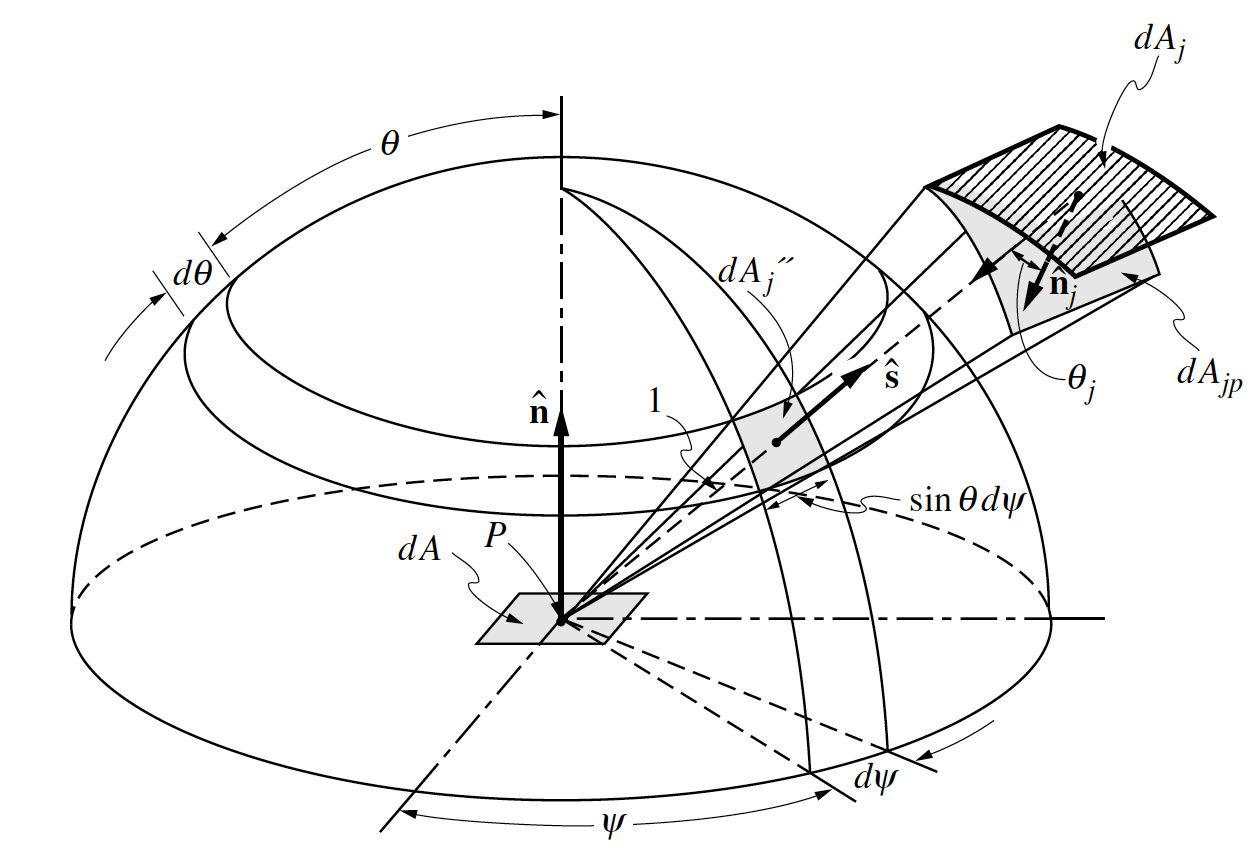
\includegraphics[width=0.7\linewidth]{figures/ch3/solid_angl.png}
\caption{Angle definitions for ray direction from a boundary. $\theta$ is the polar angle and ranges from $0$ to $\pi/2$. $\psi$ is the azimuthal angle and ranges from $0$ to $2\pi$. When a ray is emitted from a point in a medium, a ray may be emitted in any direction across the unit-sphere, and $\theta{}$ will range from $0$ to $\pi$.}
\label{fig:Unit_Sphere}
\end{figure}
Local thermodynamic equilibrium guarantees isotropic emission; therefore, the directions can be calculated as
\begin{equation}
    \psi{} = 2\pi{}R_\psi{}~\text{and}
    \label{eq:DirOfEmission_psi}
\end{equation}
\begin{equation}
    \theta{}=\arccos{(1-2R_\theta{})}~.
    \label{eq:DirOfEmission_theta}
\end{equation}
Note the non-linear dependence of polar direction on the uniformly distributed random variable, unlike the naive approach defined previously.

\subsubsection{Absorption}
The spectral absorptivity $\alpha{}_\eta{}$ of ray in a non-scattering medium follows as one minus Beer's law, as
\begin{equation}
    \alpha{}_\eta{}=1-\exp{\left(-\int^{t}_0\kappa{}_\eta{}~ds\right)}~,
    \label{eq:transmissivity}
\end{equation}
where $t$ is the distance the ray has traveled. The random number relation for the absorption location of the ray can be defined as
\begin{equation}
    R_{abs}=\exp{\left(-\int_0^{t}\kappa_\eta{}~ds\right)}
    \label{eq:discreteabsorption}
\end{equation}
which may be reformulated for ray traversal through a series of $N$ discrete sub-volumes, where complete ray absorption will occur at $N$th intersected cell as
\begin{equation}
    R_{abs}=\exp{\left(-\sum{}_{i=1}^N\kappa_\eta{}\Delta{}s_i\right)}~\text{, or}
\end{equation}
\begin{equation}
    \sum{}_{i=1}^N\kappa_{i\eta{}}\Delta{s_i}=\ln{\frac{1}{R_{abs}}}~,
    \label{eq:discreteabsorption_cells}
\end{equation}
where $\Delta{s}_i$ is the distance travelled through cell $i$.

As mentioned in section~\ref{section:RTE}, the absorption coefficient may vary unpredictably along its path length. As a result, the change of a ray's intensity requires knowledge of the ray's current intensity (i.e. requires some knowledge of the ray's \textit{history} during traversal).  
Therefore, with the exception of the null-collision method (see section \ref{section:reformulations}), a ray must be traced through the mesh sequentially in order to accurately determine the deposited energies. In other words, the summation term in Eq.~\ref{eq:discreteabsorption_cells} is incrementally evaluated from its emission point until the addition of the $N$th cell has exceeded the right hand side, at which point cell $N$ will absorb the ray in its entirety.

Alternatively, the absorption process can also be modeled using the energy partitioning approach where Eq. \ref{eq:transmissivity} is used directly in discrete form to define the gradual depletion of ray intensity. 
In forward MCRT, each cell that a ray intersects will receive an energy defined by the difference of ray energy at the entrance and exit of the cell. Then, the ray's propagation will continue until its energy has depleted below a threshold value.
The energy partitioning approach is known to be more efficient in an optically thin medium where the rays will propagate far in the domain before complete absorption~\cite{Modest2013RadiativeTransfer,Liu2020TheFlames}, and is employed in this research.

\subsubsection{Wavelength}
The random number relation for the wavelength can be described as
\begin{equation}
    R_\eta{}=\frac{\pi{}}{\kappa{}_p\sigma{}T^4}\int_0^\eta{}\kappa{}_\eta{}I_{b\eta{}}~d\eta{}~.
    \label{eq:RN_relation_wavelength}
\end{equation}
% While the preceding relations for point of emission and direction of emission can be assumed uniform within a computational cell and isotropic with direction, respectively, the same uniformity cannot be assumed for the ray's wavelength. 
For most mixtures in combustion modeling, the radiative emission spectrum varies significantly as a function of wavelength due to the highly intermittent modes of oscillation within the gas particles (see section \ref{Sec:Nongray}). 
Therefore, the inversion process of Eq. \ref{eq:RN_relation_wavelength} is complex.
Adaption of the most accurate non-gray model in radiation, the line-by-line model, to MCRT requires a spectroscopic database such as HITEMP~\cite{Rothman2010HITEMPDatabase} to integrate Eq.~\ref{eq:RN_relation_wavelength}. 

In this research, the inversion of Eq.~\ref{eq:RN_relation_wavelength} follows the multi-step procedure defined by \citet{Ren2013AGases}. This procedure exploits the additive nature of radiative emission, where the net volumetric radiative emission per unit solid angle $E_{tot}$ can be determined by summing the contribution of each emitting species, as
\begin{equation}
    E_{tot} = \sum_{i=1}^{n_s}\int_0^\infty{}{\kappa{}_{\eta{}i}I_{b\eta}~d\eta}~,
    \label{eq:Net_emission_by species}
\end{equation}
for $n_s$ emitting species. The inversion of Eq.~\ref{eq:RN_relation_wavelength} may then proceed by first determining the emitting species $s$ according to
\begin{equation}
    s=j \qquad \text{if} \qquad \frac{\sum\limits_{i=1}^{j-1}E_i}{\sum\limits_{i=1}^{n_s}E_i} < R_\eta \leq \frac{\sum\limits_{i=1}^{j}E_i}{\sum\limits_{i=1}^{n_s}E_i}~,
\end{equation}
rescaling the random number as
\begin{equation}
    R_{\eta{}s}=\frac{R_\eta{}E_{tot}-\sum\limits_{i=1}^{j-1}{E_i}}{E_j}~,
\end{equation}
and evaluating the emitting wavenumber by inverting the emission spectrum for just the emitting species,
\begin{equation}
    R_{\eta{}s}=\frac{\pi}{\kappa_{ps}\sigma{}T^4}\int_0^\eta{}{\kappa_{\eta{}s}I_{b\eta}~d\eta}~.
    \label{eq:RN_wavelength_by_species}
\end{equation}
This approach is not only more efficient, but also allows for an explicit determination of the chemical species that emits a ray.

To invert Eq.~\ref{eq:RN_wavelength_by_species}, the approach used in this research is to create a table of wave-numbers and their corresponding integrated emissive powers $E_{partial}$, 
\begin{equation}
    E_{partial}=\int_0^\eta{}{\kappa_{\eta{}s}I_{b\eta}~d\eta}~.
\end{equation}
The table is created by incrementally increasing the $\eta{}$, calculating the integrated emissive power, and tabulating the data. As $\eta{}$ approaches wavenumbers of order $15000~cm^{-1}$, the integral approaches the total emissive power of $\kappa{}_{ps}I_b$, and the integration is concluded. Prediction of wavenumber given an emitting species is then determined by multiplying the species-specific random number $R_{s\eta}$ by the total emissive power extracted from the last index in the table, and finding the wavenumber that corresponds to that partial emissive power.

\subsection{Raytracing}\label{section:Raytracing}
The conventional MCRT methods rely on a raytracing procedure to determine the optical distances a ray propagates through in each cell, as shown in Fig.~\ref{fig:raytracing}. 
The ray energy modeled using Eq.~\ref{eq:transmissivity} requires knowledge of the order of cell intersection, as well as the distance travelled through each cell, $\Delta{}s$. While many structured meshes can evaluate tracing procedures using a fast pre-computing approach~\cite{Amanatides1987ATracing}, unstructured meshes, like those used in \texttt{OpenFOAM}, require tracing through one cell at a time to determine the sequence of cells intersected.
Therefore, the traditional approach to raytracing is to incrementally trace the ray through the mesh, one cell at a time in order of intersection, using the exit faces of one cell to determine the next cell that is intersected. 

Algorithm~\ref{alg:traditional_raytracing} defines a traditional forward Monte Carlo approach to MCRT. First, each cell is given an allotment of rays that are responsible for redistributing the radiative emissive power of that cell, defined by variable $emitting\_cell.rays$, and each ray is initialized using the random number relations from section~\ref{section:randomnumberrelations}. The number of rays emitted can either be a uniform value ranging from $1$ to $1000$, or defined using the emissive power of that cell as in the adaptive emission approach, see section~\ref{section:adaptiveemission}. Then, each ray is traced through the mesh while its energy is greater than a certain minimum threshold. Each iteration of the while loop starts with the trigonometric calculation to determine the distance propagated through the cell $\Delta{s}$. Then, the spectral absorption coefficient $\kappa_\eta$ for the ray is determined given the thermodynamic state of the cell (pressure, temperature and chemical species composition) as well as the ray's wave-number $\eta$. Provided this information, the spectral optical distance traversed within the cell $\tau{}_\eta{}$ is calculated, and the ray's energy is depleted in accordance with Beer's law, as on line~\ref{lst:line:beerslaw}. The depleted energy from the ray is deposited into the $cell.E$ to model radiative absorption. Finally, the exit face of the current cell is used to determine the next cell intersected for the next iteration of the while loop.



The procedure requires calculations between every ray (up to tens of millions) and every cell that each ray intersects (up to several thousands). 
Due to the exceedingly high number of ray-cell interactions that must be computed, raytracing is often responsible for the bulk of the runtime consumed by the MCRT method~\cite{Humphrey2012RadiationSystem} (see Fig.~\ref{fig:Sample_Profiling}). As such, particular attention is dedicated to ensuring these calculations are as efficient as possible in the present MCRT code.
\begin{figure}
\centering
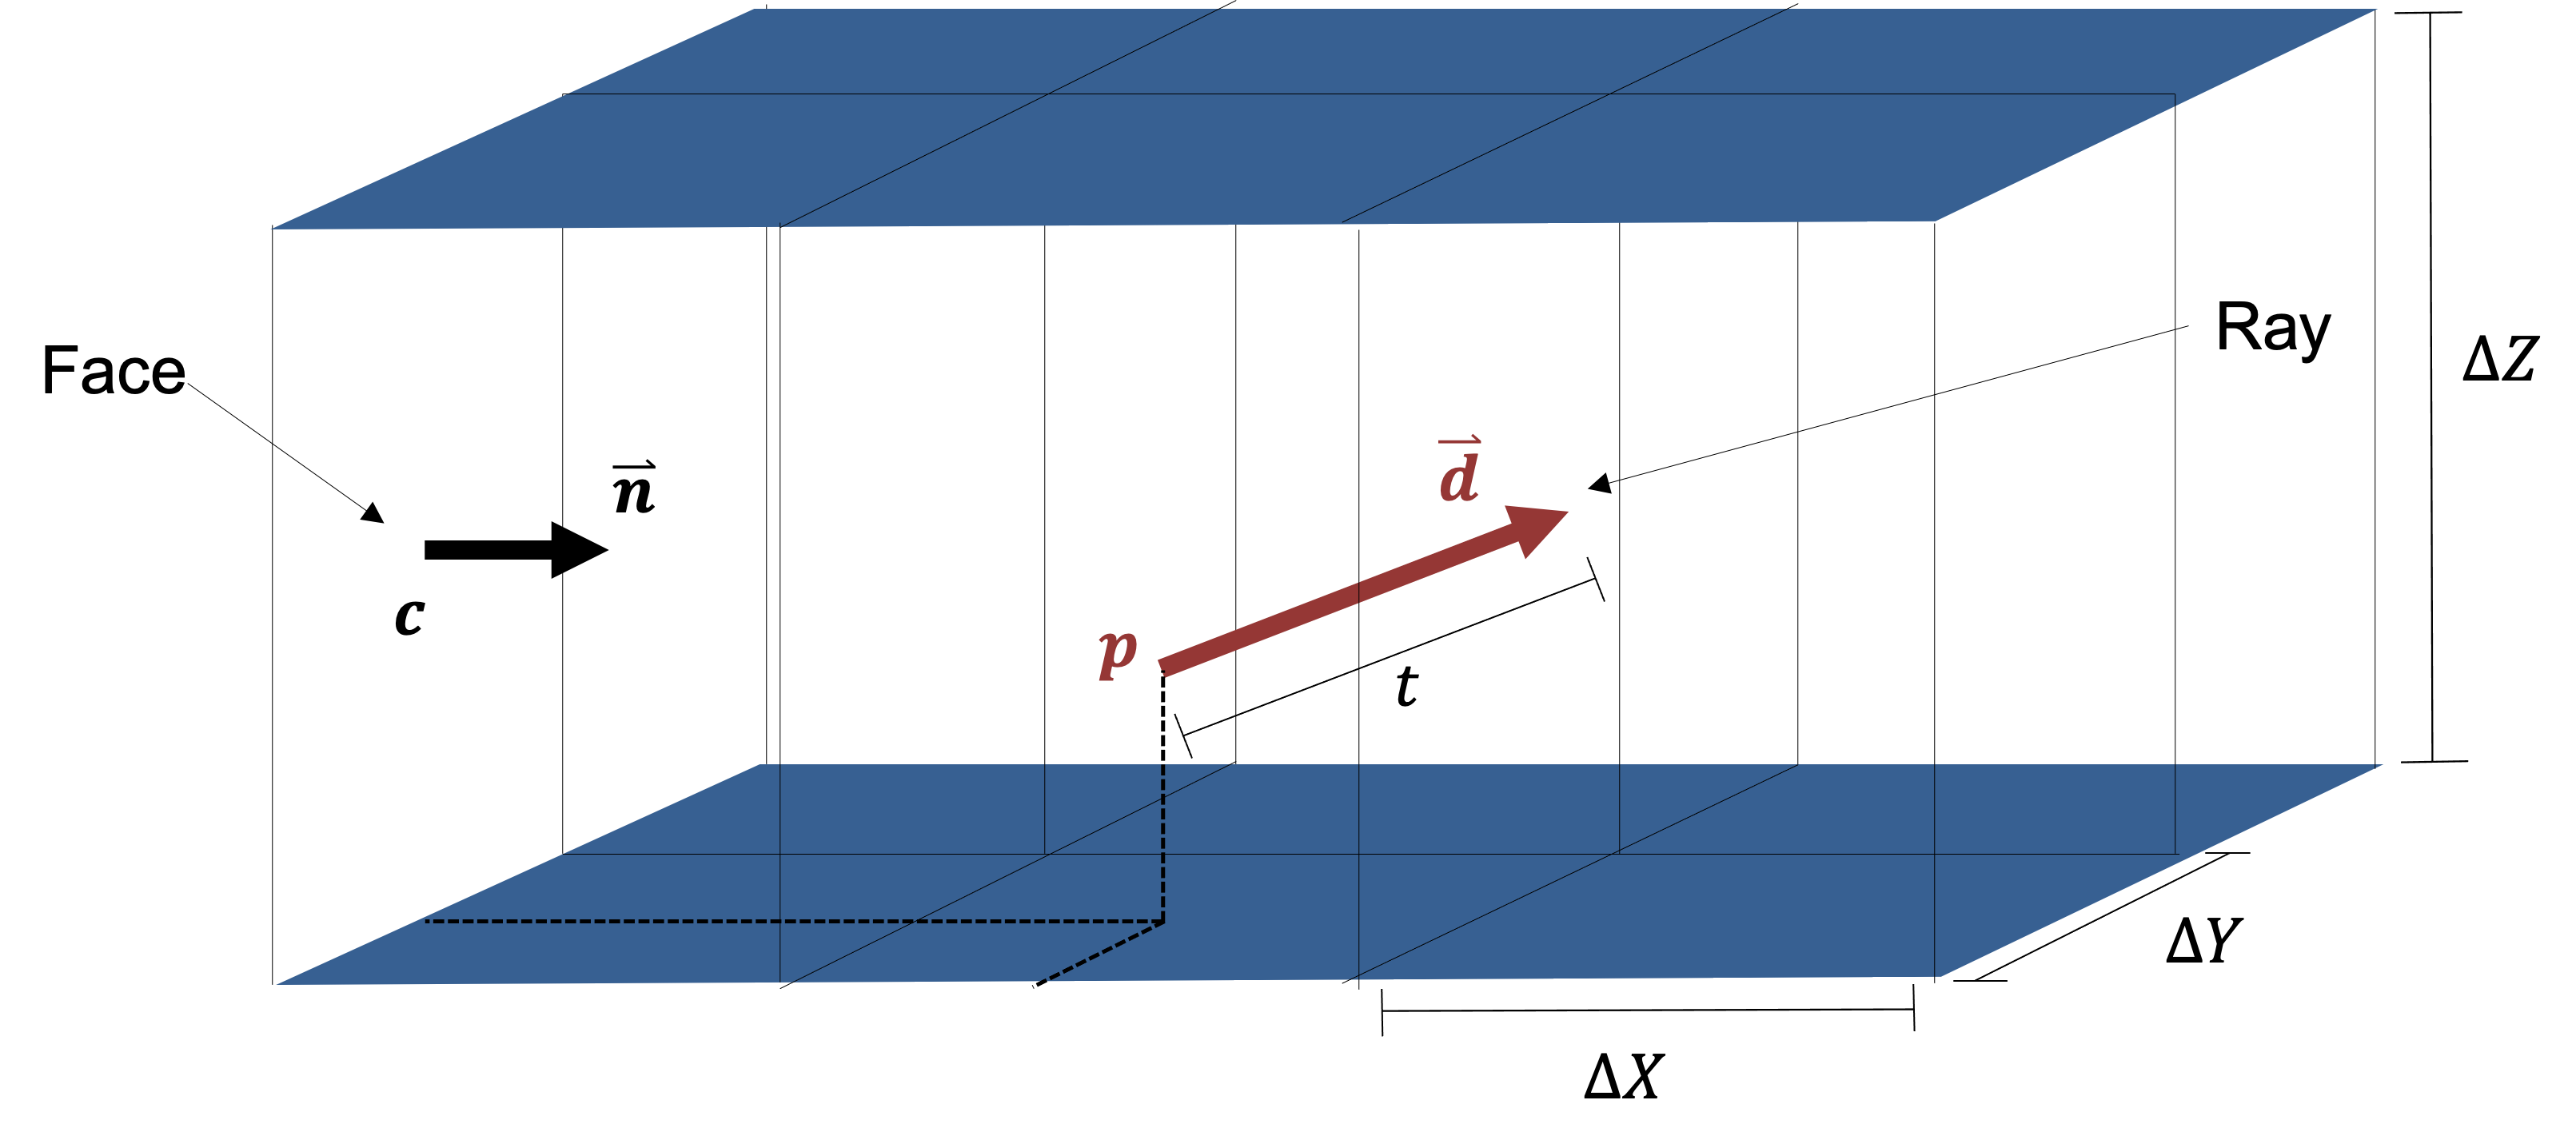
\includegraphics[width=0.8\linewidth]{figures/ch3/TracingThroughMesh.png}
\caption{Visual depiction of a ray traveling through a mesh. }
\label{fig:raytracing}
\end{figure}


\begin{algorithm}
    \caption{Pseudocode for the traditional ray tracing process through a mesh. No ray-boundary interactions, ray scattering, or parallel processing is accounted for.}
    \label{alg:traditional_raytracing}
    \begin{algorithmic}[1] % The number tells where the line numbering should start

        \Procedure{Raytracing}{$mesh$}
            \For{$emitting\_cell \in{} mesh$}
                \For{$ray \in{} emitting\_cell.rays$}
                    \State \Call{Ray.Initialize}{~} \Comment{point of emission, direction, wavelength}
                    \State $cell\gets emitting\_cell$
                    \While{$ray.energy > energy\_minimum$}\label{lst:line:energymin}
                        \State $\Delta{s} \gets \Call{ray.get\_intsec\_length}{cell}$
                        \State $\kappa{}_\eta{} \gets \Call{cell.get\_absorption\_coeff}{ray.wavenumber}$
                        \State $\tau_\eta{} \gets \Delta{s}\times{\kappa{}_\eta{}}$ \Comment{optical distance}
                        \State $E_{temp} \gets ray.E$ 
                        \State $ray.E \gets ray.E * \exp{(-\tau_\eta)}$ \label{lst:line:beerslaw}
                        \State $cell.E \gets cell.E + (E_{temp} - ray.E)$
                        \State $cell \gets \Call{ray.get\_next\_cell}{ }$
                    \EndWhile
                \EndFor
            \EndFor
        \EndProcedure
        
    \end{algorithmic}
\end{algorithm}



\subsubsection{Trigonometric Calculations}
Determining the distance travelled within a cell, $\Delta{s}$, requires calculations involving the ray and each of the faces of the cell~\cite{Zeeb2001AnGeometries}.
The calculation proceeds as follows. Upon initialization, the ray is located within its originating cell. Within an arbitrarily shaped polyhedral cell, the exit face of the ray can only be determined by iterating through each face.
While iterating through each face, the ray's intersection point along the face's plane is first calculated, then it is determined if the exit point lies within the boundaries of the face.

To evaluate the distance before interesecting the face, the following procedure is employed. The point of a ray $\textbf{r}$ with direction $\Vec{\textbf{d}}$ and origin $\textbf{p}$ after propagating a distance of $t$ along its path length can be calculated as
\begin{equation}
    \textbf{r} = \Vec{\textbf{d}}t + \textbf{p}~.
    \label{eq:ray_equation}
\end{equation}
Meanwhile, the equation of a plane with a normal vector $\Vec{\textbf{n}}$ (which faces the exterior of the cell) and center-point $\textbf{c}$ can be represented as
\begin{equation}
    \Vec{\textbf{n}} \cdot (\textbf{r} - \textbf{c}) = 0~.
    \label{eq:eq_for_plane}
\end{equation}
Substituting Eq. \ref{eq:ray_equation} into Eq. \ref{eq:eq_for_plane} creates the expression for the distance the ray travels before intersecting the plane $t_{int}$,
\begin{equation}
    t_{int}=\frac{d-\Vec{\textbf{n}}\cdot\textbf{p}}{\Vec{\textbf{n}}\cdot\Vec{\textbf{d}}}~,
    \label{eq:eq_for_t}
\end{equation}
where $d=\Vec{\textbf{n}}\cdot\textbf{c}$, and can be pre-computed before the ray tracing procedure begins~\cite{Kay1986RayScenes}. The calculation of $t_{int}$ is conducted with each face of the cell to determine the exit face. When the dot product of a ray's direction with the face norm $\Vec{\textbf{n}}\cdot{}\Vec{\textbf{d}}$ is negative, it is known that the face cannot be the exit location of that ray and the face should be skipped. If the dot product is positive, the point of intersection of the ray is then calculated using Eq.~\ref{eq:ray_equation}.


Next, it is confirmed whether the ray's exit point exists within the bounds of the face. For this, Sunday's winding number algorithm is applied~\cite{Sunday2021PracticalCode}. This algorithm determines whether a point falls within a two-dimensional polygon of arbitrary shape. The algorithm can be extended for use in three dimensions by ignoring the normal vector coordinate of highest magnitude, and applying the point-in-face test using the other two coordinates.


Finally, assuming the cells are contiguous in space, the exit face of the cell is used to determine the entrance face of the following cell using conveniently defined mesh arrays.
The procedure then repeats as discussed in the previous section until the ray has depleted sufficiently (falls below $energy\_minimum$ on line~\ref{lst:line:energymin}), or until a boundary has been intersected.

\subsubsection{Boundary Interactions}
%The boundary interactions are dependent on the boundary conditions defined within the model. 
% Five types of boundary conditions are considered in the solver: wall, symmetry, processor boundary, inlet/outlet and cyclic.
Three types of boundary conditions are considered in the solver: wall, symmetry and processor boundary. Processor boundaries are applied when the boundary represents the interface with the computational cells situated on another computing process, or MPI rank. When a ray intersects this type of boundary, it is later communicated to the rank for continued tracing.
For wall interaction, two models are commonly implemented in MCRT: black boundaries and gray boundaries.
A black surface is one that absorbs all incident radiation and emits according to Planck's law, Eq.~\ref{eq:PlancksLaw} in section~\ref{section:BasicLaws}. 
This type of boundary could be used to represent a combustor boundary or an opening to the surroundings (by assigning the boundary a constant, cold temperature). 
When a ray intersects a black boundary it is absorbed fully. Emission from a black surface is diffuse, and therefore directions of emissions are defined by the random number relations for a diffuse, emitting surface, as
\begin{equation}
    \psi{}=2\pi{}R_\psi\text{, and}
    \label{eq:diffuse_emission_psi}
\end{equation}
\begin{equation}
    \theta = \arcsin{\sqrt{R_\theta}}~.
    \label{eq:diffuse_emission_theta}
\end{equation}

A gray boundary has a more complex interaction with the environment. Gray surfaces can absorb, transmit, and reflect incident radiation. Gray surfaces also have only a fraction of the emission as that of a black body.
The transmissivity $\tau{}$ quantifies the fraction of incident radiation that passes through the surface, the absorptivity $\alpha$ is defined as the fraction of incident radiation that is absorbed, and the reflectivity $\rho$ is the fraction that is reflected. These definitions can be re-stated for a non-ideal, rough surface by replacing the -ivity suffix with -ance. 
Finally, from the emission perspective, the emissivity $\epsilon$ is the ratio of boundary's emissive power to that of a black body.  Kirchoff's law (see section \ref{sec:KirchoffsLaw}) indicates that $\epsilon{}=\alpha{}$ under the conditions of radiative equilibrium.
For opaque and gray surfaces, the reflectivity can be determined by the relation $\rho{}=1-\epsilon$, where knowledge of the emissivity is sufficient to determine a boundary's reflectivity because $\tau{}=0$.

\begin{figure}
\centering
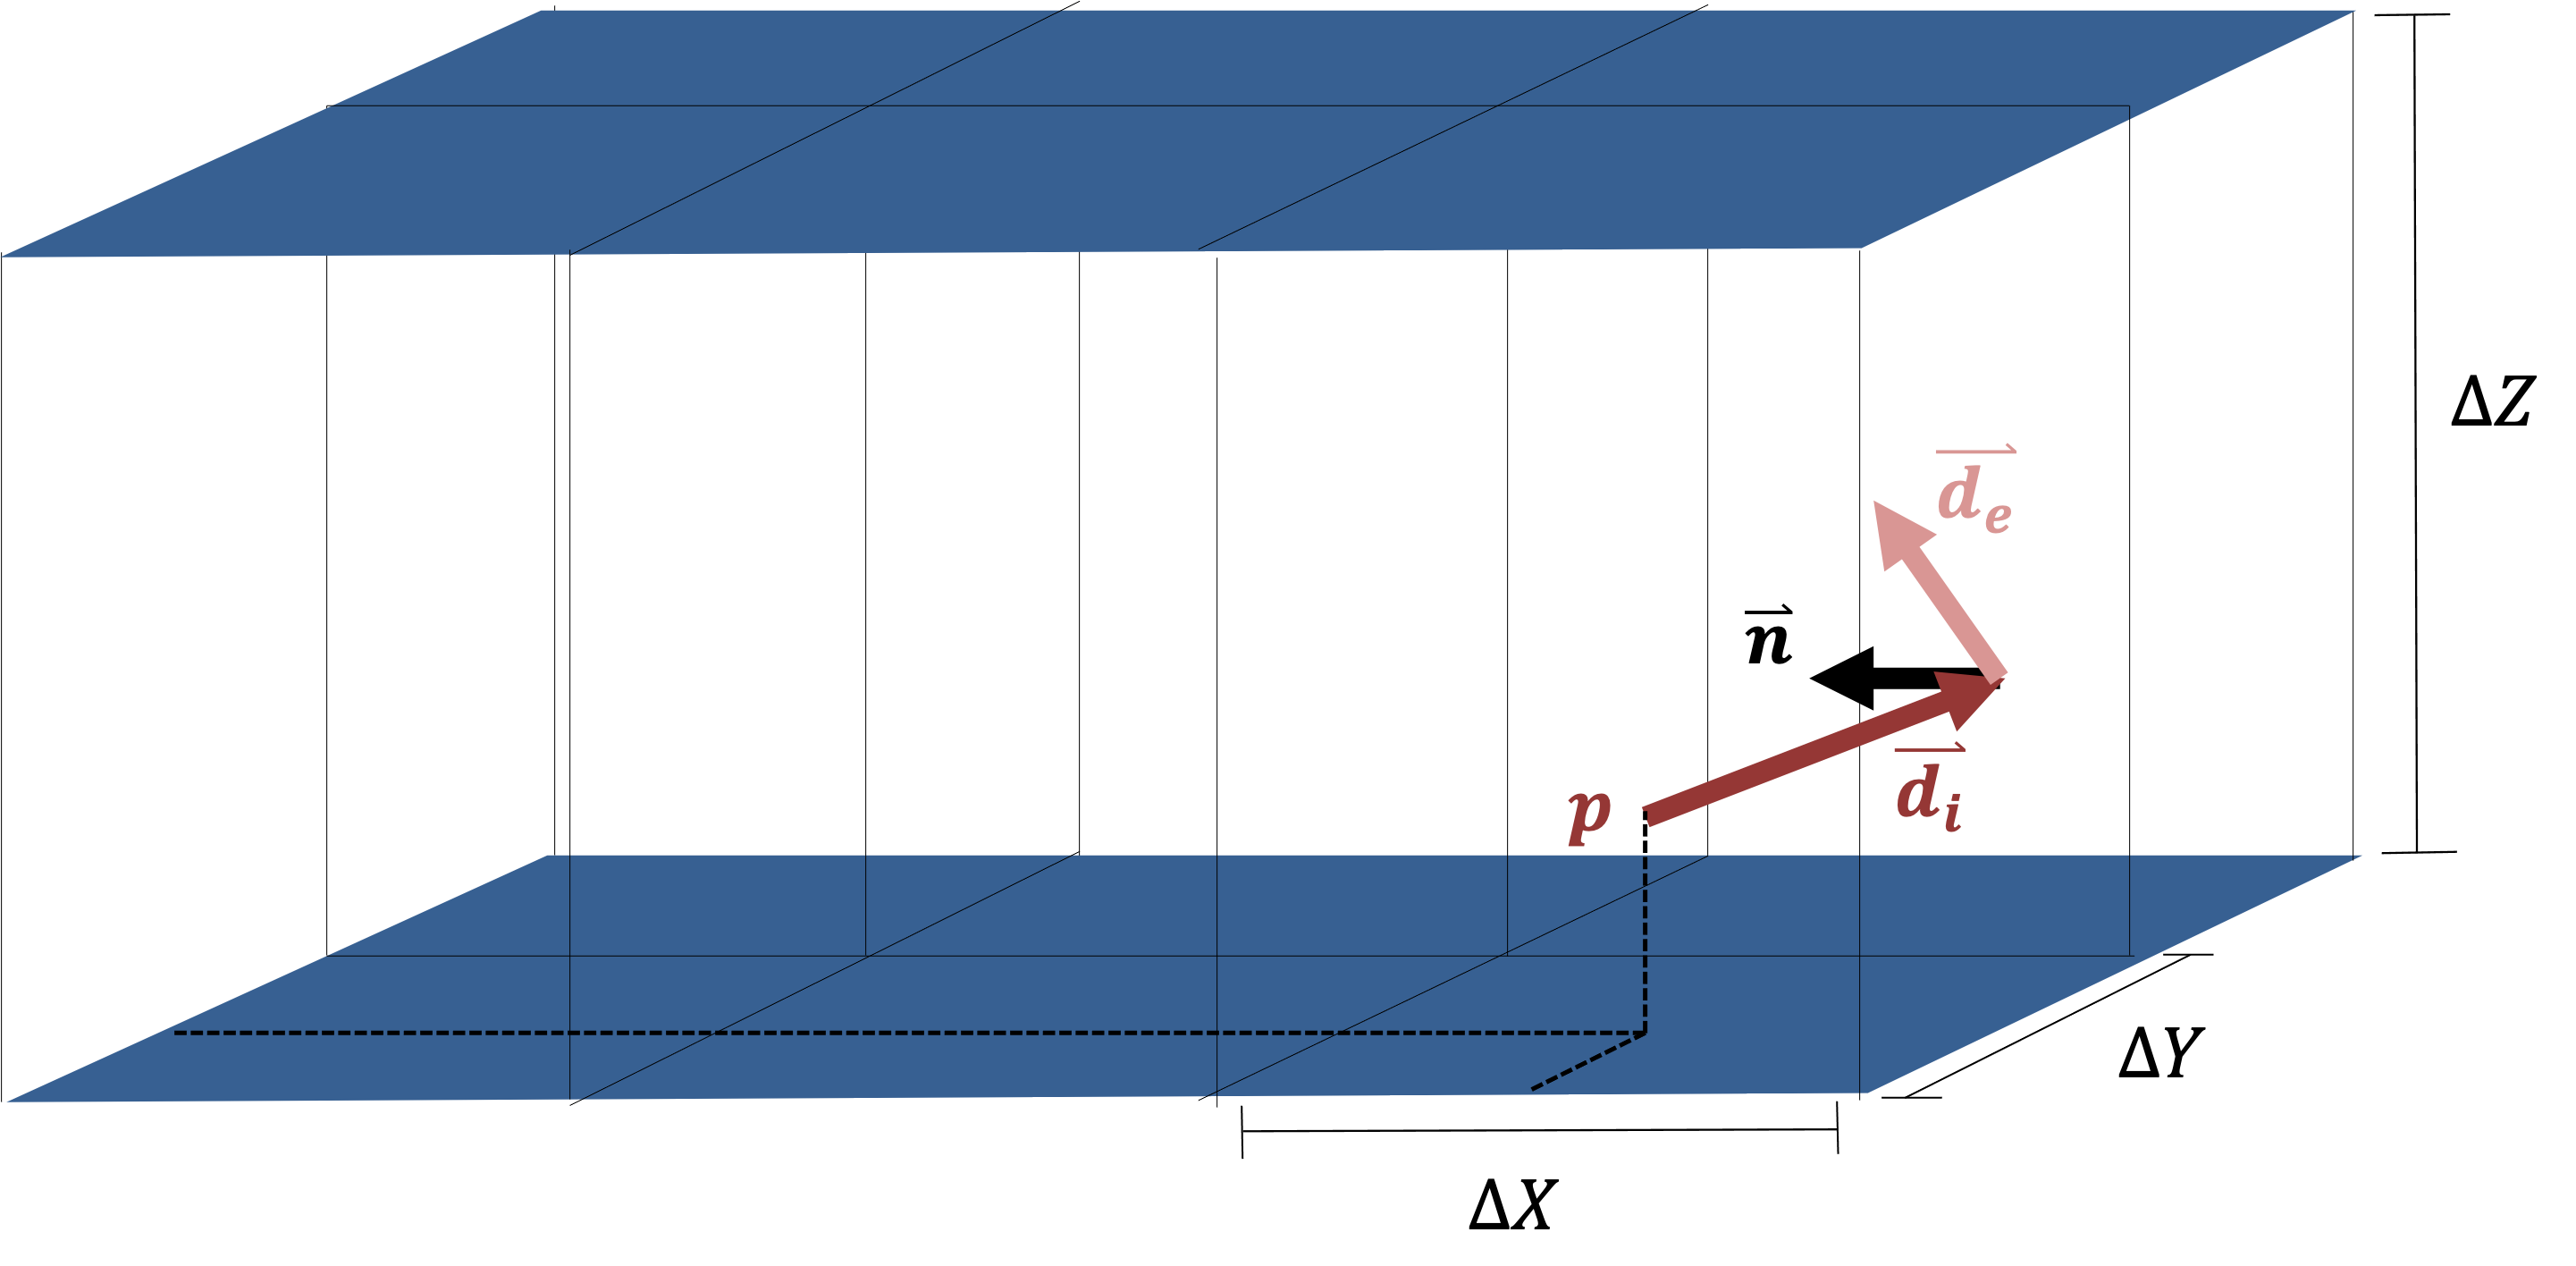
\includegraphics[width=0.8\linewidth]{figures/ch3/SpecularReflection.png}
\caption{Visual depiction of a specular ray reflection. }
\label{fig:specularreflection}
\end{figure}

Reflecting boundaries redirect incident rays from a wall-incident direction to a wall-exiting direction. 
The exit direction can be evaluated using either a \textit{diffuse} or \textit{specular} model. 
A diffuse reflection occurs when an incident ray is deflected back in a random direction into the medium. This is accurate for surfaces with a high degree of variability of surface norms (rough surfaces), and the exit direction can be evaluated using Eqs. \ref{eq:diffuse_emission_psi} and \ref{eq:diffuse_emission_theta}.
A specular reflection is one that occurs from a smooth material, and can be visualized as Fig.~\ref{fig:specularreflection}. 
An example would be a mirror or the smooth surface of water. Under these conditions, the wall-exit direction can be calculated as
\begin{equation}
    \Vec{\textbf{d}_e}=2(\Vec{\textbf{n}}\cdot\Vec{\textbf{d}_i})\Vec{\textbf{n}} -\Vec{\textbf{d}_i}~,
    \label{eq:specular_reflection}
\end{equation}
where $\Vec{\textbf{d}_{e}}$ is the exit direction, $\Vec{\textbf{d}_i}$ is the incident direction, and $\vec{\textbf{n}}$ is surface norm. During this process, the ray's wavenumber remains constant, but the energy will decrease to a fraction $\rho$ of its original energy.
Symmetry boundaries also can be described by this specular reflection.


% \subsection{Turbulence Modeling}
% The modeling of disparate time and length scales involved with turbulent fluctuations in many fluid dynamic systems presents a problem for many computational scientists.
% Resolving all of these scales would require extremely well resolved grid, often to an infeasible degree computationally. 
% Instead, a coarser grid is often used, with properties defined by an average over that of the contained fluid structures. This is the approach used in Reynold's Averaged Navier Stokes (RANS) modeling and Large Eddy Simulations (LES).
% The averaging of the governing equations of fluid dynamics; however, presents another difficulty, as many non-linear terms are contained which may complicate the averaging procedure.
% This problem emerges in turbulent modeling of radiation, and is often called Turbulence-Radiation Interaction (TRI).

% The transport of radiation can be divided into processes of emission and absorption. 
% Within a semi-transparent medium, or any surface-surface exchange of radiation, the emission and absorption are defined by a non-linear functions of the thermodynamic conditions in the medium.
% Equation~\ref{eq:DivHeatFlux} is the divergence of heat flux due to radiation. It defines the contribution of radiation to a differential volume, and its negative represents the volumetric energetic source term in the energy equation for fluid dynamics.
% \begin{equation}
%     -S_{rad}=\nabla\cdot{}q_{rad} = \int_0^\infty{\left(4\pi{}\kappa_\eta{}I_{b\eta{}}-\int_{4\pi}{\kappa{}_\eta{}I_\eta{}~d\Omega{}}\right)~d\eta{}}
%     \label{eq:DivHeatFlux}
% \end{equation}
% The averaging process will reformulate the equation into the following, eq.~\ref{eq:AvgDivHeatFlux}.
% \begin{equation}
%     -S_{rad}=\langle\nabla\cdot{}q_{rad}\rangle = \int_0^\infty{\left(4\pi{}\langle\kappa_\eta{}I_{b\eta{}}\rangle-\int_{4\pi}{\langle\kappa{}_\eta{}I_\eta{}\rangle~d\Omega{}}\right)~d\eta{}}
%     \label{eq:AvgDivHeatFlux}
% \end{equation}
% The simple change introduces a significant complexity into the system. The distinction can be described as
% \begin{equation}
%     \text{Absorption TRI:~~}\langle\kappa_\eta{}I_{\eta}\rangle \neq \kappa_\eta{}(\langle\phi{}\rangle) I_{\eta}(\langle{}T\rangle{})~, and
%     \label{eq:AbsTRI}
% \end{equation}
% \begin{equation}
%     \text{Emission TRI:~~}\langle\kappa_\eta{}I_{b\eta}\rangle \neq \kappa_\eta{}(\langle\phi{}\rangle) I_{b\eta}(\langle{}T\rangle{})~,
%     \label{eq:EmiTRI}
% \end{equation}
% where $\phi{}$ is a vector defining the thermodynamic state and chemical composition of the mixture. Therefore, absorption and emission TRI refers to the modeling technique used to estimate the left-hand side terms in Eqs.~\ref{eq:AbsTRI} and~\ref{eq:EmiTRI}, respectively.

% As a simple demonstration, the total intensity emitted from a black-body is defined by Eq.~\ref{eq:PlancksLawIntegrated} and~\ref{eq:Intensity}.
% An apparent relationship between the emission and $T^4$ captures the first problem, as $\langle{T}\rangle^4 \neq \langle{}T^4\rangle$. 
% The consequences of which may be conceptualized easily. Many turbulent combustion systems exhibit a high degree of fluctuations in temperature. Even within the length-scale of a computational cell, a flame-thickness may be small enough that there may exist a pocket of product mixture alongside an cooler, unburnt gas.
% Therefore, one can expect a higher degree of emission than predicted after an evaluation of $\langle{T}\rangle^4$, a phenomenon which presents itself when comparing radiation from a fully resolved Direct Numerical Simulation (DNS) and averaged simulations (RANS, LES) with no TRI~\cite{Modest2016RadiativeSystems}.
% Similar arguments can be made regarding the influence of the absorption coefficient on emission, as it is also a nonlinear function of chemical composition and temperature.
% The influences of $T$ and $\kappa{}_\eta{}$ on emission are categorized as emission TRI.

% Identically, absorption TRI accounts for the non-linearities within the the components of absorption. Unfortunately, absorption TRI requires modeling of not only the local absorption coefficient, but also the intensity across all solid angles throughout the unit sphere.
% The all-to-all nature of radiation means that the irradiation fluctuates as a function of emission fluctuations everywhere in the medium, as well as absorption fluctuations between all of those places and the point of interest. Fortunately, absorption TRI can often be neglected according to the Optically Thin Fluctuation Assumption (OTFA), which says that fluctuations of local absorption are only weakly correlated to fluctuations elsewhere, and therefore the left and right hand sides of Eq.~\ref{eq:AbsTRI} can be assumed equal.

% The importance of TRI modeling has been recognized for many years, and numerous methods have been proposed to account for its contribution. Extensive reviews have been created such as that of \citet{Modest2016RadiativeSystems} and \citet{Coelho2018RadiativeSystems}. For the results presented in Chapter~\ref{chapter:Example} the influences of TRI are assumed negligible. All cases presented are either highly resolved and don't require sub-grid modeling, or are homogeneous cases.

\section{Accelerated approaches to MCRT}

\subsection{Adaptive Emission Model}\label{section:adaptiveemission}
Oftentimes, only a small number of computational cells within a combustion-CFD domain have high temperatures and therefore high degrees of radiative emission. Under these circumstances, a uniform emission model, where the number of rays emitted from each cell is the same, will result in a large number of rays with small amounts of energy. These rays may contribute a significant computational expense while contributing little information to the overall RTE solution.
The adaptive emission model is a solution to this problem. In this approach, the number of rays emitted from each computational cell is decided by the emissive power of that cell~\cite{Wang2007AnFields}.
Given a user-defined target number of rays $N_{rays,tot,target}$, the target ray-energy can be calculated as 
\begin{equation}
    E_{ray,target}=\frac{\sum^{N_{cells}}_{i}E_{i}}{N_{rays,tot,target}}~,
    \label{eq:TargetRayEnergy}
\end{equation}
where $E_i$ is the emissive power from cell $i$ and $N_{cells}$ is the total number of cells in the mesh. 
Given this target ray-energy, the number of rays emitted from any given cell $j$ can be calculated as
\begin{equation}
    N_{rays,cell,actual}=\left\lceil{\frac{E_{i}}{E_{ray,target}}}\right\rceil{}~,
    \label{eq:NumberOfRays}
\end{equation}
and the actual ray energy as
\begin{equation}
    E_{ray,actual}=\frac{E_{i}}{N_{rays,cell,actual}}~.
    \label{eq:RayEnergies}
\end{equation}

\subsection{Monte Carlo reformulations}\label{section:reformulations}
The forward Monte Carlo method is the most common implementation of MCRT and is useful to provide knowledge of the overall radiation field~\cite{Modest2022ChapterMediac}. However, alternative methods have been proposed that provide unique advantages under various circumstances.
Many of these methods rely on an inversion of the radiation problem, so rays can be traced back to their point of origin, a concept that relies on the reciprocity principle of radiation~\cite{Case1957TransferPrinciple}.

\subsubsection{Backwards/Reverse Monte Carlo}
It is often necessary to evaluate the incident radiation upon a point or small surface, such as a radiometer or a motion detector.
Applying the forward-MC approach would result in be an exhaustive calculation, as only a small portion of the rays would reach the point of interest. It would be more convenient to exclusively compute rays which are known in advance to arrive at that point. 
Backwards Monte Carlo provides a more efficient route for this type of problem.
Instead of tracing rays from their points of emission, rays are instead traced backwards from their points of absorption.
Instead of allocating ray energies based on the emitting computational cell, rays are instead backtracked from the "destination cell", back through their "emission cells", while accumulating the energy emitted from each cell along the way. After a sufficient optical distance, it is reasonable to assume that no significant radiation would be contributed from any further radiation along the path length, and the accumulated intensity of the ray is deposited into the "destination cell". 
This approach is common in radiation modeling, and can be applied to transient radiative transfer problems~\cite{Lu2004ReverseMedia} and semi-transparent media~\cite{Li2005BackwardSlab}.

The BMC (backwards Monte Carlo) approach is based on the principle of reciprocity approach formally derived by~\citet{Case1957TransferPrinciple} and expanded to participating media by~\citet{Walters1992RigorousMedia}.
Further background regarding the method can be found in texts by~\citet{Modest2003BackwardTransfer} and~\citet{Howell2010ThermalTransfer}.

The RTE, Eq. \ref{eq:RTE_Solution}, can be inverted for to calculate intensity at a point $\textbf{r}_i$ and direction $-\hat{s}_i$ as
\begin{equation}
    \begin{aligned}
    I_\eta{}(\textbf{r}_i,-\hat{s}_i) =~&\epsilon{}_\eta{}(r_w)I_{b\eta{}}(r_w)\exp{\left[-\int_0^l\kappa{}(r')~dl'\right]}\\
    &+\int_{0}^{l}{ \left\{ \kappa_\eta(r')I_{b\eta}(r')\exp{\left[-\int_0^{l'}\kappa_\eta(r'')~dl''\right]} \right\}}~dl'~,
    \label{eq:Inverted_RTE}
    \end{aligned}
\end{equation}
where $l$ defines the distance along the ray's path. Equation \ref{eq:Inverted_RTE} provides a method to solve the RTE in a reverse manner.
Assuming piece-wise homogeneity, Eq. \ref{eq:Inverted_RTE} can be reformulated into
\begin{equation}
    \begin{aligned}
    I_\eta{}(\textbf{r}_i,-\hat{s}_i)& = \epsilon{}_\eta{}(r_w)I_{b\eta{}}(r_w)\exp{\left[-\sum_{m=1}^M\kappa{}_{\eta{},m}(l_{m_{out}}-l_{m_{in}})~\right]}\\
    &+\sum_{m=1}^M\left( I_{b\eta}(T_m)\left\{ \exp{\left[-\sum_{p=1}^{m_{in}}\kappa{}_{\eta{},p}(l_{p}-l_{p-1})\right]}- \exp{\left[-\sum_{p=1}^{m_{out}}\kappa{}_{\eta{},p}(l_{p}-l_{p-1})\right]} \right\} \right)~.
    \end{aligned}
    \label{eq:discrete_Inverted_RTE}
\end{equation}
for $M$ intersected cells along the ray's path. Equation~\ref{eq:discrete_Inverted_RTE} can then be solved in stochastic form using the Monte Carlo method.

Equation~\ref{eq:discrete_Inverted_RTE} offers a physical description of the back-tracking of a ray.
As the ray travels in the reverse direction, it passes through a series of computational cells. 
As the ray is traced, each intersected computational cell contributes a portion of the net energy deposited to the ray's originating cell. The energetic contribution of each of the passing cells is accounted for alongside a transmissivity term to determine their contribution's decay before arriving at the originating cell.
After tracing a multitude of ray samples, the net radiative absorption within the originating cell is evaluated as
\begin{equation}
    E_{abs}=~\frac{4\pi{}\kappa_p}{N_{rays}}\sum_j^{N_{rays}}I_j(\textbf{r},\textbf{s}_i)~.
    \label{eq:RMCRT_Absorption}
\end{equation}

% From a computational point of view, reverse Monte Carlo can also improve the memory footprint of MCRT.

\subsubsection{Reciprocal Monte Carlo}
Reciprocal Monte Carlo\footnote{Also referred to as direct-exchange MC in the text by~\citet{Modest2022ChapterMediac}.} is a variance reduction technique that relies on evaluations of the net exchange of power between two computational cells or surfaces.
Following~\citet{Howell2020ThermalTransfer}, a close look at the forward and reverse Monte Carlo methods discussed previously reveals that the first law of thermodynamics is enforced by ensuring that the energy emitted from one computation cell and deposited to another computational cell will be equal values. However, the second law of thermodynamics is only imposed stochastically. This is evident when considering the exchange of energy between cells. The second law states that there should be a net energy exchange from a cell of higher temperature to a cell of lower temperature. For the discussed methods so far, this rule may be violated when the higher temperature cell does not emit a statistically significant number of rays that intersect the lower temperature cell, or vice-versa.
The approach in the reciprocal Monte Carlo implementation is to embed the requirement of both first and second law satisfaction in the model; as a result, reciprocal Monte Carlo theoretically has lower variance compared to the forward and reverse Monte Carlo methods~\cite{Howell2020ThermalTransfer}. 

Several implementations of reciprocal Monte Carlo methods have been proposed by~\citet{Tesse2002RadiativeApproach} and~\citet{Dupoirieux2006AnThicknesses}. These include the Emission reciprocity method (ERM), absorption reciprocity method (ARM), and a hybrid of the two, optimized reciprocity method (ORM).

A complete solution to the RTE would require the evaluation of all power exchanges, $P_{i,j}^{exch}$, between every pair of surfaces and cells $(i,j)$ in the domain.
The net power exchange for one particular object $P_q$ can thereafter be evaluated as the sum of net power exchange with every other object as
\begin{equation}
    P_q=\sum_{j=1}^{N_v+N_S}P_{qj}^{exch}=-\sum_{j=1}^{N_v+N_S}P_{jq}^{exch}~,
    \label{eq:power_exchange}
\end{equation}
where $N_V$ and $N_S$ are all of the volumes and surfaces within the geometry, and
$P_{ab}$ defines the net power exchange from object $b$ into object $a$.
ERM and ARM differ in which term they attempt to estimate: ERM estimates the first summational term of Eq.~\ref{eq:power_exchange}, and ARM estimates the second summational term of Eq.~\ref{eq:power_exchange}.
In ERM, the estimated value for a spectral power exchange from a volume $j$ into a volume $q$ can be evaluated as
\begin{equation}
    P_{qj\eta}^{ERM}=4\pi{}\kappa_{q\eta}V_q(I_{bj\eta}-I^0_{bq\eta})A_{qj\eta}~,
    \label{eq:fraction_spectralpower_ERM}
\end{equation}
where the spectral power exchange can be related to the net power exchange as $P_{qj}^{exch}=\int_0^\infty{}P_{qj\eta}^{exch}~d\eta$.
Meanwhile, for ARM, the exchange is evaluated as
\begin{equation}
    P_{jq\eta}^{ARM}=4\pi{}\kappa_{j\eta}V_j(I_{bq\eta}-I^0_{bj\eta})A_{jq\eta}~.
    \label{eq:power_exchange_ARM}
\end{equation}
$A_{jq\eta}$ represents the fraction of spectral power emitted by cell $j$ that is absorbed by cell $q$, and often requires a stochastic solution using the Monte Carlo method. Additional formulations for $A$ between surfaces, and surfaces and volumes can be found in~\citet{Dupoirieux2006AnThicknesses}.

\citet{Dupoirieux2006AnThicknesses} later presented a mathematical description of the variance of the two procedures ERM and ARM. It was determined that the standard deviation of ERM is lower than that of ARM when the temperature $T_q$ is larger than $T_j$, and conversely ARM is more precise under the opposite condition.
Therefore, the procedure conducted in ORM is to select which to evaluate at runtime for every pair exchange by comparing the relative temperatures between the two objects.

With the net power exchange being evaluated instead of the one-sided contribution of one cell to other cells (forward MC), and from other cells into one cell (backward MC), the total number of ray histories being tracked through one tracing procedure is increased.
Therefore, the information obtained through one tracing of reciprocal MC is generally greater than that of the other presented approaches.

\subsubsection{Null-collision Monte Carlo}
The null-collision Monte Carlo method applies a Russian-roulette approach to MCRT.
The descriptions of the MCRT methods presented so far have implied that it is necessary to trace a ray through the CFD mesh.
This requirement exists for determination of either ray energy depositions (forward MC), emission contributions (backward MC), or power exchange (reciprocal MC). 
The reason for tracing originates from the expected variability of extinction coefficient $\beta{}_\eta{}$ along a ray's path. 
This variability is nearly guaranteed; the spatial inhomogeneity of the system's temperature, pressure, chemical composition all results in spatial in-homogeneity of the ray's extinction coefficient. 
The ray must be traced through each computational cell to explicitly evaluate the interaction of the ray with that cell.
However, if one could assume homogeneity in $\beta{}_\eta{}$, no mesh tracing procedure would be required. The interaction of the ray with the surrounding medium could be assumed uniform along the ray's travel.
This is the intention behind the null-collision algorithm~\cite{Galtier2013IntegralAlgorithms,Eymet2013Null-collisionSimulators}.

The principle of null collision is to redefine the extinction coefficient as,
\begin{equation}
    \beta{}_\eta{} = \kappa{}_\eta{}+\sigma{}_\eta+\kappa{}_{\eta{},null}~,
    \label{eq:null_coll_absco}
\end{equation}
where an additional null-collision coefficient $\kappa{}_{\eta,null}$ has been introduced in addition to the absorption coefficient $\kappa{}_\eta$ and scattering coefficient $\sigma{}_\eta{}$. 
The value of this coefficient is defined as the exact value that allows for $\beta{}_\eta{}$ to remain constant throughout the ray's travel.
The random number relation for extinction, from Eq. \ref{eq:discreteabsorption_cells}, is 
\begin{equation}
    \tau_{extinct} = \ln{\frac{1}{R_\beta{}}}~.
    \label{eq:discreteabsorption_cells_repeated}
\end{equation}
and the length propagated before ray extinction, $s_{ext}$ is evaluated through inversion of
\begin{equation}
    \tau_{ext,\eta{}} = \int_0^{s_{ext}}{\beta{}_\eta{}~ds}~.
    \label{eq:randomextinctionlength}
\end{equation}
Usually, the inversion of Eq. \ref{eq:randomextinctionlength} requires tracing through the mesh, as mentioned previously, to calculate the change in $\beta_\eta$. However, with the introduction of the null-collision coefficient $\beta{}_\eta{}$ is no longer a function of $s$ and can be removed from the integral and Eq. \ref{eq:randomextinctionlength} can be simplified to $\tau{}_{ext,\eta}=\beta{}_\eta{}s_{ext}$. Therefore, inversion may be completed analytically as $s_{ext}=\tau{}_{ext,\eta}/\beta{}_\eta{}$.
 
With this change, the tracing procedure may proceed as follows. When the ray is first initialized, the optical distance before extinction is randomly determined using Eq. \ref{eq:discreteabsorption_cells_repeated}, and the resulting extinction distance, $s_{ext}$, is evaluated analytically using $s_{ext}=\tau{}_{ext,\eta}/\beta{}_\eta{}$.
After the ray has travelled this distance, a new absorption coefficient and scattering coefficient are determined, and a random number, $R$ is drawn again.
The random number is used in a round of Russian-roulette.
The ray is terminated if $R<\kappa{}_\eta{}/\beta{}_\eta{}$, scattered if $\kappa{}_\eta{}/\beta{}_\eta{}<R<(\kappa{}_\eta{}+\sigma{}_\eta{})/\beta{}_\eta{}$ and continues propagation if $R>(\kappa{}_\eta{}+\sigma{}_\eta{})/\beta{}_\eta{}$. 
The null collision event can therefore be thought of as a scattering event, but with no change in direction.

Null-collision was re-introduced to the field of stochastic modeling of radiation and graphics rendering by~\citet{Galtier2013IntegralAlgorithms}. Since then, null-collision has see a growth in usage as an alternative to the traditional approach of tracing through a grid. 
Various interpretations of the algorithm are offered by~\citet{ElHafi2021ThreeAlgorithms}, each revealing a new perspective and application for the method.
The method has been applied under a variety of circumstances with recent extensions to Monte Carlo evaluation of spectroscopic parameters~\cite{Galtier2015RadiativeApproach}, Oct-tree methods for an optimal evaluation of extinction locations~\cite{Villefranque2019AAtmospheres}, and combustion simulations~\cite{Eymet2013Null-collisionSimulators}.


\subsection{MPI acceleration}\label{section:MPIacceleration}
The all-to-all nature of MCRT results in poor scaling with increasing mesh size. 
With large enough simulations, the system geometry is divided into separate regions that are computed on different computers, called nodes, on a high performance computing system. When the ray-tracing procedure begins, rays must be traced through the mesh on one node before being communicated to another node for continued tracing.
Ray-cell interactions may occur between a ray emitted on one side of the medium, and a cell located on the other side.
The resulting communication overhead required by the Message Passing Interface (MPI)\footnote{MPI is the parallel execution standard for distributed memory computers. It defines the syntax in C/C++/Fortran code used to communicate with other nodes in the high performance computer (HPC).}, can dramatically slow the computation. Additionally, the sequential nature of raytracing limits these MPI communications to an iterative sequence of communications between adjacent MPI ranks\footnote{An MPI rank, in this case, is an instance of a parallel execution process within MPI.}.
This results in a series of "MPI iterations" where rays are forced to wait at the boundary of one MPI rank before being communicated to the adjacent rank as a group. This wait time significantly reduces the performance and limits the scalability of the solver.

\subsubsection{Mesh Coarsening}
Mesh coarsening is one approach to alleviate this problem. The approach is to localize all mesh information within a node to prevent any MPI communications.
To store the full mesh on one node would violate one of the main purposes of a distributed-memory simulation, so a mesh coarsening approach is imposed, where the mesh is less-refined at increasing distances from the point of emission.
The coarsened mesh reduces the memory load required to store the mesh. Several layers can be added of increasing degree of coarsening further from node of interest. The concept capitalizes on the local nature of thermal radiation: 
while radiation can travel long distances, in many circumstances, the radiation will have its most significant contributions local to the point of emission.
The following explanation follows that of~\citet{Silvestri2019ASimulation}.

The transmitted radiative intensity through a mesh follows an exponential decay function of intersection length and absorption coefficient, proportional to
\begin{equation}
     I_{transmit} \sim \exp{\left(-\kappa{}_\eta{}\Delta{s}\right)},
    \label{eq:specular_reflection}
\end{equation}
It is immediately apparent that the majority of ray absorption occurs at lower optical distances. This suggests that a coarsening of the mesh at larger optical distances (further from the point of emission) can reduce computational runtime while maintaining a similar degree of accuracy.
The ray will be emitted and traced within the fine mesh locally, and transferred to a coarsened mesh after a prescribed number of grid steps.
Resulting, in total, for a reduced number of ray-cell calculations, and also the potential to store the entirety of the mesh on a single node, in a coarsened manor. 

The idea has been implemented a limited number of times, but with much success.~\citet{Silvestri2019ASimulation} presented speedups approximately equal to the number of coarsened layers within a structured mesh, along with an method to optimally select the number of cells a ray should travel before coarsening and obtained an order of magnitude reduction in runtime. 
\citet{Humphrey2015ATracing} applied a similar concept to a gray reverse Monte Carlo model within a structured mesh.~\citet{Kelm2021TheTransport} applied the OpenFOAM-embedded LaGrangian particle tracking library to radiation transport in their solver, \verb|containmentFoam|, which uses a global mesh to prevent MPI communications.

Several possible issues remain within the method, however. For one, the requirement of a user specified number of grid steps inserts a certain degree of potential error into the calculation. 
The model is restricted in accuracy and applicability to only those who understand its limitations. A sufficiently general model could be applied under any circumstance, without user choice.
Additionally, the model has the potential to introduce Turbulence-Radiation Interaction (TRI)-related effects into the simulations. 
Even if appropriate averaging is conducted (averaging the complete emissive power term from each cell, weighted by cell volume) the usage of a spatially-averaging model is questionable for TRI-related studies, particularly within the context of absorption-TRI.
Finally, the implementation of a non-gray modeling with such models appears to be inefficient~\cite{Humphrey2012RadiationSystem}.

\subsubsection{Distributed Raytracing}
In this research, a new technique for MCRT on multi-MPI rank simulations is presented for accelerated ray tracing. This approach reformulates the backwards Monte Carlo method presented previously to accelerate the model on distributed-memory systems.
To begin, the formulation for ray back-tracing is repeated for convenience as,
\begin{equation}
    \begin{aligned}
    I_\eta{}(\textbf{r}_i,-\hat{s}_i)& = \epsilon{}_\eta{}(r_w)I_{b\eta{}}(r_w)\exp{\left[-\sum_{m=1}^M\kappa{}_{\eta{},m}(l_{m_{out}}-l_{m_{in}})~\right]}\\
    &+\sum_{m=1}^M\left( I_{b\eta}(T_m)\left\{ \exp{\left[-\sum_{p=1}^{m_{in}}\kappa{}_{\eta{},p}(l_{p}-l_{p-1})\right]}- \exp{\left[-\sum_{p=1}^{m_{out}}\kappa{}_{\eta{},p}(l_{p}-l_{p-1})\right]} \right\} \right)~.
    \end{aligned}
\end{equation}
This formulation can be rewritten as,
\begin{equation}
    \begin{aligned}
    I_\eta{}(\textbf{r}_i,-\hat{s}_i)& = \epsilon{}_\eta{}(r_w)I_{b\eta{}}(r_w)\exp{\left(-\sum_{m}^{e_1\rightarrow{}e_{N+1}}\tau{}_{\eta{},m}~\right)}\\
    &+\sum_{m}^{e_1\rightarrow{}e_{N+1}}\left\{ I_{b\eta}(T_m)\left[ \exp{\left(-\sum_{p}^{e_1\rightarrow{}m}\tau{}_{\eta{},p}\right)}- \exp{\left(-\sum_{p}^{e_1\rightarrow{}m+1}\tau{}_{\eta{},p}\right)} \right] \right\}~,
    \end{aligned}
\end{equation}
where $\tau{}_{\eta{},m}$ is the spectral optical distance in the $m$th cell along the ray's path, $e_1$ is the emitting computational cell, $e_i$  is the entrance computational cell in $i$th MPI rank along the ray's path, $N$ is the number of ranks intersected, and $e_1\rightarrow{}i$ represents the sequence of computational cells between the emitting computational cell up to but not including the $i$th cell intersected. This formulation is a description of the tracing of a ray accounting for the various MPI ranks, with the exception that the ray terminates at the exit point of its last MPI rank instead of at any computational cell within a rank as before. With this change, the ray tracing procedure can be described as,
\begin{equation}
    \begin{aligned}
    I_\eta{}(\textbf{r}_i,-\hat{s}_i)& = \epsilon{}_\eta{}(r_w)I_{b\eta{}}(r_w)\exp{\left(-\sum_{m}^{e_1\rightarrow{}e_{N+1}}\tau{}_{\eta{},m}~\right)}\\
    &+\sum_{n}^{N}\sum_{m}^{e_n\rightarrow{}e_{n+1}}\left\{ I_{b\eta}(T_m)\left[ \exp{\left(-\sum_{p}^{e_1\rightarrow{}m}\tau{}_{\eta{},p}\right)}- \exp{\left(-\sum_{p}^{e_1\rightarrow{}m+1}\tau{}_{\eta{},p}\right)} \right] \right\}~.
    \end{aligned}
\end{equation}
The inner sums can be made independent of all preceding MPI ranks by splitting the sum and factoring the exponential term, as
\begin{equation}
    \begin{aligned}
    I_\eta{}(\textbf{r}_i,-\hat{s}_i)& = 
    \epsilon{}_\eta{}(r_w)I_{b\eta{}}(r_w)\exp{\left(-\sum_{m}^{e_1\rightarrow{}e_{N}}\tau{}_{\eta{},m}-\sum_{m}^{e_N\rightarrow{}e_{N+1}}\tau{}_{\eta{},m}~\right)}\\
    &+\sum_{n}^{N}\sum_{m}^{e_n\rightarrow{}e_{n+1}}\left\{ I_{b\eta}(T_m)\left[ \exp{\left(-\sum_{p}^{e_1\rightarrow{}e_n}\tau{}_{\eta{},p}-\sum_{p}^{e_n\rightarrow{}m}\tau{}_{\eta,p}\right)}\right.{} \right.{} \\
    &\quad \left.{}\left.{} -\exp{\left(-\sum_{p}^{e_1\rightarrow{}e_n}\tau{}_{\eta{},p}-\sum_{p}^{e_n\rightarrow{}m+1}\tau{}_{\eta{},p}\right)} \vphantom{\frac12}\right] \vphantom{\frac12}\right\}~\text{, and}
    \end{aligned}
\end{equation}
\begin{equation}
    \begin{aligned}
    I_\eta{}(\textbf{r}_i,-\hat{s}_i)& = 
    \epsilon{}_\eta{}(r_w)I_{b\eta{}}(r_w)\exp{\left(-
\sum_{m}^{e_1\rightarrow{}e_{N}}\tau{}_{\eta{},m}~\right)}\exp{\left(-\sum_{m}^{e_N\rightarrow{}e_{N+1}}\tau{}_{\eta{},m}~\right)}\\
    &+\sum_{n}^{N}\exp\left(-\sum_{p}^{e_1\rightarrow{}e_n}\tau{}_{\eta{},p}\right)\sum_{m}^{e_n\rightarrow{}e_{n+1}}\left\{ I_{b\eta}(T_m)\left[ \exp{\left(-\sum_{p}^{e_n\rightarrow{}m}\tau{}_{\eta,p}\right)}\right.{} \right.{} \\
    &\quad \left.{}\left.{} -\exp{\left(-\sum_{p}^{e_n\rightarrow{}m+1}\tau{}_{\eta{},p}\right)} \vphantom{\frac12}\right] \vphantom{\frac12}\right\}~,
    \end{aligned}
\end{equation}
where $\exp\left(-\sum_{p}^{e_1\rightarrow{}e_n}\tau{}_{\eta{},p}\right)$ has been separated from the interior summational term. The entire equation for $I_\eta{}(\textbf{r}_i,-\hat{s}_i)$ may then be represented as a function of three components
\begin{equation}
    \begin{aligned}
    I_\eta{}(\textbf{r}_i,-\hat{s}_i)& = 
    I_{bndry}\exp\left(-\sum_l^{N}\tau{}_{\eta{},l}\right)+\sum_{n}^{N}I_{cont,n}\exp\left(-\sum_l^{n-1}\tau{}_{\eta{},l}\right)~.
    \end{aligned}
    \label{eq:NewRMCRTintensity}
\end{equation}
$I_{bndry}$, $\tau{}_{\eta{},l}$, and $I_{cont,n}$ are the intensity contribution from the boundary, the optical distance traversed through rank $l$, and the intensity contribution from rank $n$ without consideration of the decay of that contribution before reaching the absorbing cell, respectively. These three terms are defined as:
\begin{equation}
    I_{bndry}=\epsilon{}_\eta{}(r_w)I_{b\eta{}}(r_w)\exp{\left(-\sum_{m}^{e_N\rightarrow{}e_{N+1}}\tau{}_{\eta{},m}~\right)}~,
    \label{eq:Ibndry}
\end{equation}
\begin{equation}
    \tau{}_{\eta{},l}=\sum_{p}^{e_n\rightarrow{}e_{n+1}}\tau{}_{\eta{},p}~\text{, and}
    \label{eq:RankOptDist}
\end{equation}
\begin{equation}
    I_{cont,n}=\sum_{m}^{e_n\rightarrow{}e_{n+1}}\left\{ I_{b\eta}(T_m)\left[ \exp{\left(-\sum_{p}^{e_n\rightarrow{}m}\tau{}_{\eta,p}\right)}
    -\exp{\left(-\sum_{p}^{e_n\rightarrow{}m+1}\tau{}_{\eta{},p}\right)} \vphantom{\frac12}\right] \vphantom{\frac12}\right\}~.
    \label{eq:IntContrWithoutDecay}
\end{equation}
With this change, both Eqs.~\ref{eq:RankOptDist} and~\ref{eq:IntContrWithoutDecay} are each functions of only the cells local to an MPI rank. Therefore, each MPI rank may calculate these terms asynchronously for a given ray. Subsequently, the originating MPI rank of a ray may iterate the $\tau{}_{\eta,l}$ and $I_{cont,n}$ terms from each MPI rank to evaluate the net accumulated intensity Eq.~\ref{eq:NewRMCRTintensity} which is deposited into the originating cell of the ray. The advantages of this approach are discussed further in section~\ref{section:SummaryOfSolvers}.


\subsection{Ray Tracing in computer graphics}\label{section:ComputerGraphicsTracing}
Many improvements to ray tracing have been introduced in recent years capitalizating on advancements in computational hardware and algorithms.
These improvements have largely been focused in the field of computer graphics, owing in large part to the dramatic increase in the desire for fast and detailed visualization software~\cite{Gupta2020CUDAComputing}. 
The vast knowledge obtained through extensive work to accelerate ray-tracing would be of significant value to many heat transfer researchers, but has historically been ignored~\cite{Howell2021TheTransfer}. 
In particular, the increased involvement of the Graphics Processing Unit (GPU) has resulted in dramatic boosts in computational efficiency, but has been used relatively few times in radiation modeling.
Additionally, the bounding volume hierarchy (BVH) provides a optimal data structure to accelerate the geometric search procedure of the ray-tracing process.

\subsubsection{Graphics Processing Units (GPUs)}
GPUs offer high throughput for highly parallelizable, compute-bound problems.
GPUs differ from Central Processing Units (CPUs) because of the increased attention to hiding latency through raw data parallelism as opposed to minimizing cache access time~\cite{Caulfield2009WhatsGPU}. 
This Single Instruction Multiple Data (SIMD) approach is optimized because the GPU structure has more area dedicated to the data processing as opposed to the cache and control unit on the CPU~\cite{Gupta2020CUDAComputing}.
At its origin, the GPU was used for the acceleration of graphical visualization of games and animation rendering. Today, GPUs are applied in vast number of fields for more general purposes (GPGPUs).

Computational scientists in particular have begun to take advantage of GPUs in their fields of study. In the hybrid computing model, a central processing unit (CPU) offloads compute-intensive and time consuming parts of the code to the GPUs.
By applying this model, users can selectively offload the necessary parts of the code to the GPU, while maintaining others on the CPU.

While many fields have seem considerable improvements with GPUs, thermal radiation modeling has seen them applied relatively few times. This comes as a surprise seeing that MCRT in particular carries many similarities to the ray-tracing in computer graphics \cite{Zeeb2001AnGeometries}.
Alerstam et al.~\cite{Alerstam2008ParallelMigration} applied GPUs to accelerate their modeling of photon migration in biomedical optics and observed over three orders of magnitude speedup over CPU implementations. Heymann et al.~\cite{Heymann2012GPU-basedAGN} applied GPUs to accelerate their ray tracing in galactic nuclei and observed speedups of over $100$ times over serial code. Humphrey et al.~\cite{Humphrey2012RadiationSystem} applied heterogeneous computing for their combustion CFD code, using GPUs for ray tracing and CPUs for combustion modeling. They recently extended their code to use the \texttt{Kokkos} programming model~\cite{Trott_Kokkos3_2022} and achieved $80$ times speedup using GPUs~\cite{Holmen2017ImprovingTasks}. Finally, Silvestri and Pecnik~\citep{Silvestri2019ASimulation} applied GPUs to their non-gray code for coupling to turbulent flow calculations and observed speedups approaching three orders of magnitude.

\subsubsection{Bounding Volume hierarchy}
At its simplest form, the bounding volume hierarchy (BVH) is a tree-based data structure which can be used to represent a series of objects in space~\cite{Shirley2020RayWeek,Meister2021ATracing}. The usage in computer graphics is to detect intersections between a ray and a far-away object with logarithmic algorithm time complexity (traversal through a tree), rather than linear time complexity (test each object one at a time)~\cite{Zeeb2001AnGeometries}.

BVHs are constructed by first wrapping the objects, e.g., surfaces in a graphical visualization, in Axis Aligned Bounding Boxes (AABBs). In a cartesian coordinate system, the box cornerpoints can be determined using the maximum and minimum X, Y, and Z coordinates of the object.
This ensures that an intersection of the ray with the object cannot occur without an intersection of the ray with the bounding box, and the detection of ray/box intersections is extremely fast~\cite{Kay1986RayScenes}.
The object-level AABBs represent the leaf nodes of the binary tree. These boxes are then wrapped in larger bounding-boxes, and the procedure repeats until there is one bounding box which wraps around the whole domain, which represents the root node of the BVH. 
For a binary tree, each node must have only two child nodes. The ray-tracing procedure can then proceed iteratively down the tree, rejecting nodes and their children that the ray does not intersect, until a final list of leaf nodes are left.

Graphics processing exhibits massive speedup with the use of the BVH data structure, especially with recent approaches using GPUs~\cite{Nery2013ParallelGPGPUs,Meister2021ATracing,Karras2012MaximizingTrees}.
However, BVHs see almost no usage in thermal radiation modeling~\cite{Liu2020TheFlames}.
\citet{Kuczynskia2014RadiationBoundaries} for one, were able to accelerate computation of thermal radiation between faces with non-participating media. 
Also,~\citet{Mazumder2006MethodsTransport} compared the BVH approach with a spatial-partitioning approach known as volume-by-volume advancement and found the BVH to be slower for surface-to-surface calculations. 
There apparently exist no applications of the BVH to participating media in thermal radiation modeling. However, alternative approaches, such as the oct-tree approach where a mesh is refined in regions of increased opacity, have been introduced and shown to provide significant speedups over traditional ray tracing~\cite{Saftly2013UsingNote,Villefranque2019AAtmospheres}.

\section{Implementation for this Research} \label{section:ModelForThisStudy}
In this research we create a combined combustion CFD and Monte Carlo radiation solver named MCRT-GPU. This solver applies Graphics Processing Units and Bounding Volume Hierarchies to accelerate the ray tracing process. 
Multiple variations of the solver are implemented to assess the performance benefits of GPUs and BVHs under different configurations.
The different variations rely on either forward or reverse Monte Carlo formulations and are tested and timed in both shared and distributed-memory environments in Chapter~\ref{chapter:Example}.

\begin{figure}
  \centering
  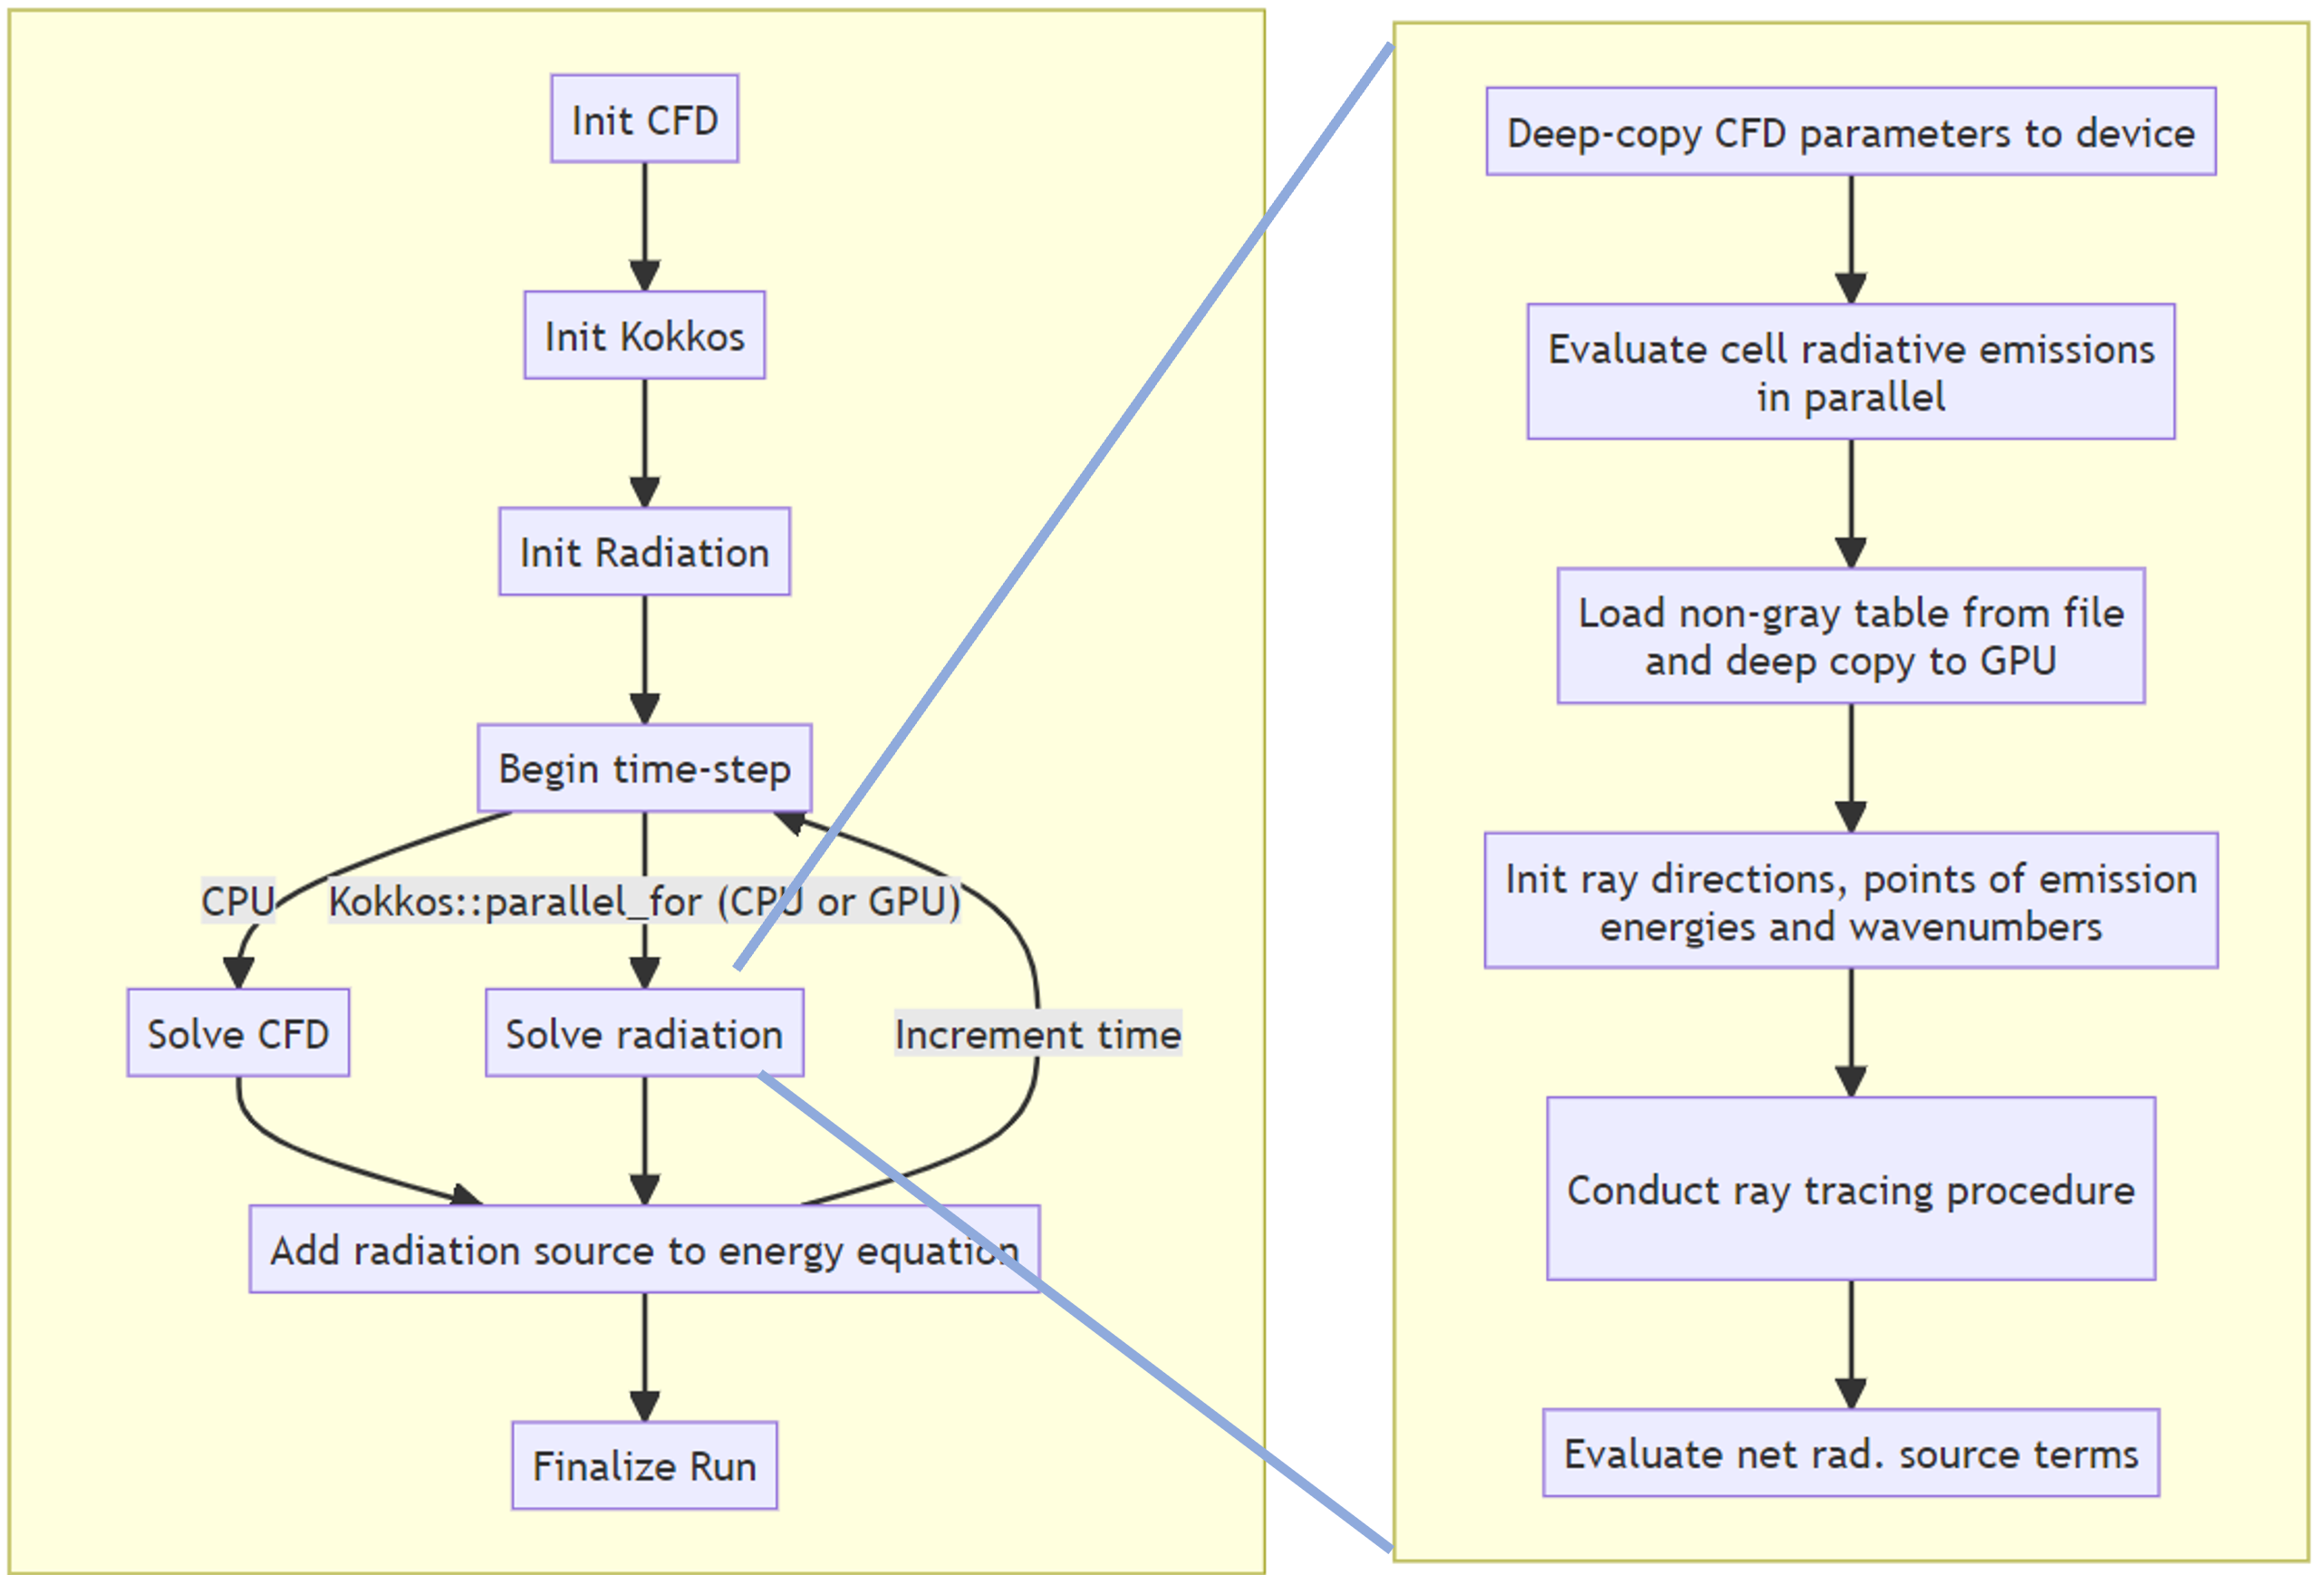
\includegraphics[width=01.0\linewidth]{figures/ch3/joint_flow_chart.png}
  \caption{Flow chart of coupled combustion-CFD and MCRT implementation. The left box refers to the overall coupled code, while the right box details the radiation solver only. The solver at its current state can solve radiation on the Kokkos device (i.e. GPU, if available, else CPU) and CFD on the CPU. A deep-copy is a data transfer from host to device. The ray tracing procedure follows the implementations listed in section~\ref{section:SummaryOfSolvers}.}
  \label{fig:joint_flow_chart}
\end{figure}

The flow chart in Fig.~\ref{fig:joint_flow_chart} provides a general summary of how the radiation solver couples to the CFD, and section~\ref{section:SummaryOfSolvers} details the ray tracing methods. The MCRT solver first reads the mesh and cell parameters from \texttt{OpenFOAM}, including temperature, pressure, and chemical species mole fractions. The radiation-relevant data are then `deep-copied' into the device-accessible memory space in preparation for the ray-tracing procedure (i.e. CPU to GPU memory transfer is conducted, if a GPU is employed). An optional line-by-line non-gray model~\cite{Ren2019Line-by-lineSystem} is included in the solver to account for the non-gray influences of the major emitting chemical species in hydrocarbon flames: CO$_2$, H$_2$O, CO, and soot.
%If the user decides to enable non-gray modeling, 
The line-by-line tables are read from a user-defined directory and deep-copied into GPU texture memory if a GPU is in use. 
%Line-by-line tabulation follows that described by Ref.~\cite{Ren2019Line-by-lineSystem}. 
\textit{Texture memory} is an NVIDIA feature that enables faster read-only memory. Alternatively, the user has the option to conduct a gray calculation using a uniform absorption coefficient or the local Planck-mean absorption coefficient. 

A parallel execution process calculates the radiative emission from each of the computational cells and delegates the emitting energy among the rays emitted from that cell. The number of rays emitted per cell may be defined manually or using the adaptive emission approach, where cells with higher radiative emission are provided more rays (see section~\ref{section:adaptiveemission}. Subsequently, the ray tracing procedure begins the asynchronous tracing of the rays using a multitude of threads.

\subsection{Supplemental Libraries}\label{section:SupplementalLibraries}
MCRT-GPU relies on several external libraries for the computation of the CFD, for a bounding volume hierarchy, and for parallelization.

\subsubsection{OpenFOAM}
By coupling to the \verb|OpenFOAM| open-sourced CFD solver, this code can be applied to any combustion application from aeronautical engines to fire suppression and management~\cite{Weller1998ATechniques}. OpenFOAM provides an extensive list of supplemental libraries, allowing the user to simulate using Reynolds Average Navier-Stokes (RANS), Large Eddy Simulation (LES), or Direct Numerical Simulation (DNS) approaches with multi-phase flow and detailed chemistry. 
Transient simulations can be implemented with MCRT-GPU on any polyhedral, unstructured mesh.
Users can adapt their own OpenFOAM solvers to use MCRT-GPU, or use the default examples for reactingFoam and fireFoam.

\subsubsection{Kokkos}
Kokkos is a performance-portable programming model from the Department of Energy~\cite{Trott_Kokkos3_2022,TrottKokkosOGPaper2014}. 
Targeted for HPCs, Kokkos provides abstractions over the parallel execution process and memory management in many solvers. By programming in Kokkos, the user can avoid the complications of the underlying parallel execution process and maintaining portability and instead focus on implementing code.
Kokkos supports CUDA, HIP, SYCL, HPX, OpenMP and C++ threads as parallel backends, which the user can easily switch between at compile time. Additionally, the \verb|Kokkos-tools| repository streamlines the debugging and profiling process~\cite{Trott_KokkosEcosystem2021}. For this solver, Kokkos::Cuda, Kokkos::OpenMP, and Kokkos::Serial back-ends are used as execution 
and memory spaces. Kokkos includes access to Cuda Unified Virtual Memory (UVM), an abstraction allowing for variables to live in CPU and GPU memory simultaneously, but it is not used in this solver due to performance drawbacks and limitations on multi-GPU computing systems.

\subsubsection{ArborX}
Following the Bounding Volume Hierarchy (BVH) description from~\citet{Karras2012MaximizingTrees}, the ArborX C++ library provides an implementation for both spatial-search and nearest-neighbor geometric search calculations using a BVH~\cite{Lebrun-Grandie2019ArborX:Library}. 
The ArborX application programming interface enables usage of the BVH through a two-step process: construction and traversal. The user can define \textit{primitives}, or underlying objects with labeled bounding-boxes, and ArborX will efficiently construct a balanced BVH around the primitives in parallel. Then, the user can define \textit{predicates} which define the operation the traversal process will be conducting (i.e. spatial or nearest query) while traversing the tree.
MCRT-GPU currently contains several code branches that apply the ArborX library to optimize the ray-tracing procedure in different ways.

ArborX uses Kokkos as a backend for on-node parallelism, and implements additional MPI functionality to extend the BVH query process across multi-node runs. Distributed memory executions proceed through an top-tree and bottom-tree approach for each MPI rank. The bottom tree of a rank consists of \textit{primitives} that are CFD cells. The bounding box for every cell is determined using the maximum and minimum X, Y, and Z coordinates of each cell; these boxes are designated leaf nodes in the BVH. 
Every pair of leaf nodes are wrapped in another bounding box defined using maximum and minimum coordinates for the pair, and those bounding boxes are then paired and wrapped in bounding boxes again. The process repeats with increasing box size until only one bounding box remains, called the \textit{scene} bounding box. 
Each MPI rank contains one scene bounding box to encompass the entire MPI rank region. The top-tree is constructed using the scene bounding boxes for all MPI ranks as primitives, and each MPI ranks contains a copy of the same top-tree.
MCRT-GPU applies ray-tracing procedure by first traversing the top-tree to determine the intersected MPI ranks by each ray. Then, the rays are MPI communicated to their destination ranks and traced using the bottom-trees. Further discussion is provided in section~\ref{section:SummaryOfSolvers}.

% \subsubsection{Non-gray model}
% MCRT-GPU has been built to enable use with one of three nongray models: line-by-line, gray modeling with a user-defined absorption coefficient, or gray modeling with planck-mean absorption coefficients. Non-gray databases have been previously derived from HITEMP~\cite{Rothman2010HITEMPDatabase} including contributions of CO$_2$, H$_2$O, and CO spectral lines.


% MCRT-GPU is meant to be an adaptable radiation model that can be quickly linked to the user's OpenFOAM solver for fast and accurate radiation modeling during their time-accurate CFD simulation.
% While the BVH may enable faster computation, in absence of proper development there exist both a version with and without its use.
% The version without applies the traditional Monte Carlo algorithms with Kokkos acceleration. This enables fast GPU-acceleration, with line-by-line non-gray modeling, ray-reflections, and distributed-memory calculation.
% Users can access the code through a public repository on github \footnote{https://github.com/nick-jt/MCRT-GPU}?.

\subsection{Summary of ray tracing procedures presented in this study}\label{section:SummaryOfSolvers}

The various implementations of the present ray tracing procedure solver are presented in Table~\ref{table:SolverImplementations}. Different variations are tested in attempt determine the optimal configuration for performance and scalability. Both forward and reverse Monte Carlo approaches are included, and all methods feature the Kokkos-embedded GPU capabilities discussed previously.

\begin{table}
\centering
\caption{Variations of the present MCRT solver algorithm. All variations rely on the Kokkos programming model for parallelization and OpenFOAM for CFD computation, while only Bounding Volume Hierarchy and Hybrid approaches use ArborX. Bold solvers are the primary tested versions.}
\begin{tabular}{c | c c c} 
 \hline
 ~ & Standard & Bounding Volume Hierarchy & Hybrid \\ [0.5ex] 
 \hline
 Forward-MC & \textbf{Standard-Forward} & ArborX-Forward & N/A  \\
 Reverse-MC & Standard-Reverse & \textbf{ArborX-Reverse} & \textbf{Hybrid-Reverse} \\
 \hline
\end{tabular}
\label{table:SolverImplementations}
\end{table}

\subsubsection{Standard-Forward}
The Standard-Forward MCRT approach is the classical implementation of MCRT and follows the description in section~\ref{section:ForwardMC} and the pseudocode presented in Algorithm~\ref{alg:traditional_raytracing}. In this model, rays are emitted from their points of emission, traced through the CFD mesh, and deposit energy as they travel. The tracing procedure follows an iterative approach where a ray's exit face in a cell determines the next cell intersected. Likewise, if run with distributed-memory parallelism, the ray's exit boundary of an MPI rank determines the next MPI rank that is intersected. Under these conditions, as discussed in section~\ref{section:MPIacceleration}, the tracing procedure for a given ray must be conducted one MPI rank at a time, and multiple MPI communications may be required before the ray is terminated.

As a whole, each MPI rank first conducts the tracing procedure for all rays emitted from within themselves. For any rays that intersect a "processor boundary", a boundary to another MPI rank, they are sorted by destination MPI rank and then MPI communicated to those ranks. Each MPI rank then traces all of the new rays internally, and the process repeats until all rays are terminated. The number of "MPI iterations" that are conducted with this approach varies depending on the number of ranks, the opacity of the medium, the boundary conditions, and the case geometry. No ray scattering events are modeled, but ray reflections and wall-absorption are included.


\subsubsection{ArborX-Forward}
ArborX-Forward is the first implementation to apply the BVH for acceleration. The ray-tracing procedure is visualized in Fig.~\ref{fig:FArborX_FlowChart}.
The process follows the traversal approach defined in the BVH discussion in section~\ref{section:ComputerGraphicsTracing} and the ArborX discussion in section~\ref{section:SupplementalLibraries} where a top tree is constructed around MPI ranks and each MPI rank's bottom tree is constructed using computational cells. Then, traversal proceeds through the top tree and then the bottom tree.

\begin{figure}
\centering
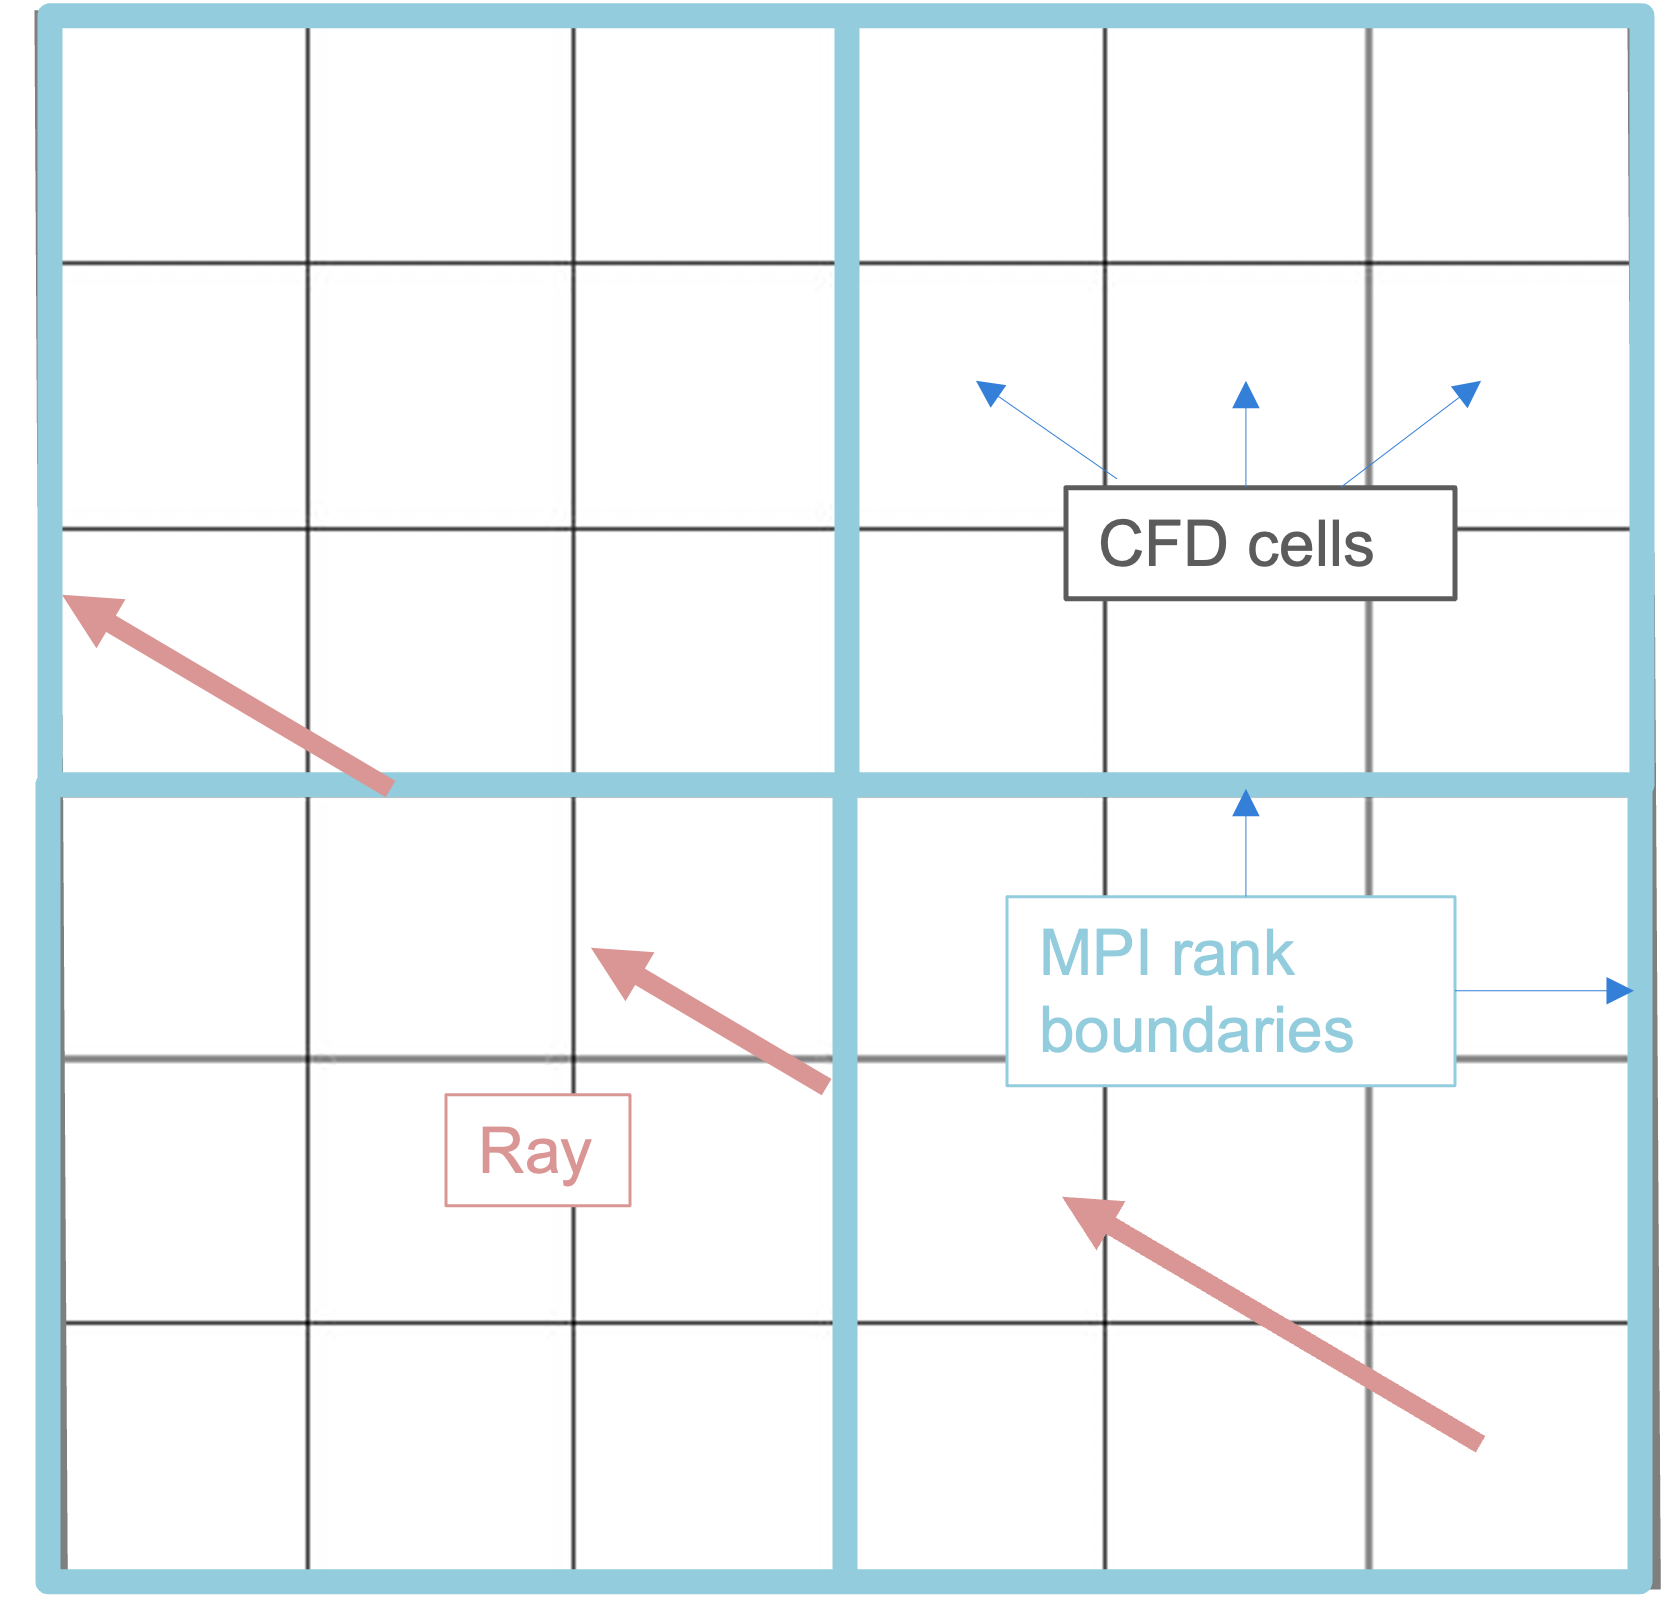
\includegraphics[width=0.5\linewidth]{figures/ch3/DistributedRayTracing.png}
\caption{A depiction of a ray being traced across multiple MPI ranks simultaneously. Within ArborX, the top-tree is constructed around MPI rank boundaries, and the bottom-trees are constructed of CFD cells.}
\label{fig:FArborX_FlowChart}
\end{figure}

For each ray, the top-tree is first traversed to determine the remote MPI ranks that a ray intersects.  Then, the rays are MPI communicated within ArborX to the remote ranks. Each MPI rank conducts a traversal of the bottom-tree to determine the computational cells that are intersected by each ray. For every ray/cell intersection that is found, a callback function is invoked to calculate the intersection characteristics of the ray with the cell using the trigonometric calculations defined in section~\ref{section:Raytracing}. The distance the ray propagated before entering the cell, the optical distance traversed within the cell, the cell's ID, the ray's ID, the ID of any intersected boundaries, and the index intersected along a boundary are then stored in a C-style struct and sent back to the originating MPI rank of the ray.
Every ray/cell intersection creates this C struct, and all of these structs are sent back to the ray's originating rank as a group. This collective send of data from every ray/cell intersection is prohibitively memory intensive, as will be discussed in Chapter~\ref{chapter:Example}. The originating rank then receives these lists of structs for each ray, and sorts them by ray intersection distance. The sorted structs are then processed in order of intersection to calculate the energy deposited by each ray to each of its intersected cells. Each MPI rank independently has knowledge of all of its rays' energetic contributions to all cells, remote and local. To sum the net radiative absorption in all cells, MPI\_AllReduce is called to conduct an all-to-all summation across every MPI rank. The storage of data for all computational cells in each MPI rank is again memory-intensive and inefficient. An improved method would not MPI\_Allreduce an array so large, and would instead only accumulate absorption for local cell data. However, due to the computational limitations imposed by the sending of ray/cell data from before, the limitations of this approach are recognized and no further effort is made for improvement.

% Send rays out to remote ranks using distributedTree. Trace rays locally using unordered-traversal (can be switched to ordered traversal easily). Communicates struct for every ray/cell intersection back to originating rank which then evaluates the net absorption for every cell. (i.e. each rank has an array that stores the absorptions for ALL cells in EVERY rank, and these arrays are MPI\_Allreduced at the end for final radiative absorptions).

\subsubsection{Standard-Reverse}
The standard-reverse tracing procedure applies the reverse Monte Carlo description presented in section~\ref{section:MPIacceleration}. In this method, rays are traced backwards from their points of absorption through emitting cells. The intensities accumulated by all rays from a cell are then averaged and integrated across the field of view ($4\pi$ steradians for a point in a medium) as shown in Eq.~\ref{eq:RMCRT_Absorption}. The random number relations and algorithm follow exactly that listed in the Standard-Forward description of section~\ref{section:ForwardMC} with the exception that the rays' accumulate energy gradually instead of deposit energy gradually.

\subsubsection{ArborX-Reverse}
The ArborX-Reverse implementation follows closely from the ArborX-Forward approach. As before, each ray on every rank is communicated to all of the MPI ranks the ray intersects using the top-tree. After communication, every rank traces each ray using the same bottom-tree traversal discussed previously.
However, in reverse ray tracing, the ray/cell interaction determines the energetic contribution of emission of the passing cell to the originating cell of the ray. Therefore, the accumulation of the intensity contribution without decay, the optical distance traversed within the rank, and the boundary intensity contribution is sufficient to predict this intensity, as shown in section~\ref{section:MPIacceleration}, and one struct is created for every ray/rank intersection rather than for every ray/cell intersection. Then, the accumulated values for every ray/rank intersection are sent back to the originating rank of the ray for evaluation of the overall accumulated ray intensity, Eq.~\ref{eq:NewRMCRTintensity}.
Finally, the net absorption within the originating cell is calculated by averaging the intensity of all of the cell's rays and integrating over the spherical solid-angle as in Eq.~\ref{eq:RMCRT_Absorption}.

\subsubsection{Hybrid-Reverse}
The hybrid approach combines standard and ArborX approaches into one. Similar to ArborX-Forward and ArborX-Reverse, Hybrid-Reverse first begins by conducting a traversal of the top-tree to determine the intersected remote ranks. However, unlike either of the two pure-ArborX approaches, the bottom-tree traversal is not conducted using the computational cells as primitives, but instead using the cell faces that fall along the MPI boundaries. 
In fact, the bottom-tree traversal only determines the first face intersected for each ray sent to a rank. This information is then used to begin a standard-reverse tracing procedure through the mesh where the exit face of the entrance cell determines the next cell intersected. The solver accumulates the values presented in Eqs.~\ref{eq:Ibndry}–\ref{eq:IntContrWithoutDecay} within one C-style struct for every ray/rank intersection, and then sends the C structs back in bulk to the originating ranks.
The originating rank then iterates through the collected structs for every ray in order of intersection and completes the evaluation of ray intensities using Eq.~\ref{eq:NewRMCRTintensity}.

% \subsubsection{NOTES}

% Can be run with Plane-parallel medium on one rank:
% \begin{itemize}
%   \item All solvers
% \end{itemize}
% Can be run with pool fire on one rank:
% \begin{itemize}
%   \item All solvers
% \end{itemize}
% Can be run with BFS on one rank:
% \begin{itemize}
%   \item All solvers
% \end{itemize}
% Can be run with multiple MPI ranks:
% \begin{itemize}
%   \item All solvers except standard-reverse and ArborX-forward
%   \item ArborX-Forward can only be used when each MPI rank has the same number of cells (i.e. the pool fires)
% \end{itemize}


% TODO: re-read GPU part, re-read everything
